\documentclass[12pt,letterpaper]{article}

% Page layout
\usepackage[margin=1in]{geometry}
\usepackage{setspace}
\onehalfspacing

% Math
\usepackage{amsmath,amssymb,amsthm,mathtools}

% Tables and figures
\usepackage{booktabs}
\usepackage{array}
\usepackage{tabularx}
\usepackage{multirow}
\usepackage{graphicx}
\usepackage{float}

% Typography
\usepackage[T1]{fontenc}
\usepackage[expansion=false]{microtype}
\usepackage{enumitem}

% References
\usepackage{xcolor}
\usepackage[colorlinks=true,linkcolor=blue,citecolor=blue,urlcolor=blue]{hyperref}

% TikZ for regime diagram
\usepackage{tikz}
\usetikzlibrary{arrows.meta,positioning,decorations.markings}

% Theorem environments
\newtheorem{theorem}{Theorem}[section]
\newtheorem{proposition}[theorem]{Proposition}
\newtheorem{lemma}[theorem]{Lemma}
\newtheorem{corollary}[theorem]{Corollary}
\newtheorem{definition}[theorem]{Definition}
\newtheorem{axiom}{Axiom}
\theoremstyle{remark}
\newtheorem{remark}[theorem]{Remark}

% Custom commands
\newcommand{\Pcycle}{P_{\text{cycle}}}
\newcommand{\FCES}{F_{\text{CES}}}
\newcommand{\phieff}{\varphi_{\text{eff}}}
\newcommand{\calF}{\mathcal{F}}
\newcommand{\calJ}{\mathcal{J}}
\newcommand{\calR}{\mathcal{R}}
\newcommand{\bone}{\mathbf{1}}
\DeclareMathOperator*{\argmax}{arg\,max}
\DeclareMathOperator{\tr}{tr}
\DeclareMathOperator{\sgn}{sgn}
\DeclareMathOperator{\diag}{diag}
\DeclareMathOperator{\Var}{Var}

% Section formatting
\usepackage{titlesec}
\titleformat{\section}{\large\bfseries}{\thesection.}{0.5em}{}
\titleformat{\subsection}{\normalsize\bfseries}{\thesubsection}{0.5em}{}
\titleformat{\subsubsection}{\normalsize\itshape}{\thesubsubsection}{0.5em}{}

\begin{document}

% -------------------------------------------------------------------
% TITLE PAGE
% -------------------------------------------------------------------
\begin{titlepage}
\centering
\vspace*{1.5cm}
{\LARGE\bfseries Complementary Heterogeneity\\[8pt]
in Hierarchical Economies\par}
\vspace{0.6cm}
{\large\itshape CES Aggregation, Derived Architecture, and\\
Cross-Sector Activation in Multi-Timescale Systems\par}
\vspace{1.5cm}
{\large Jon Smirl\par}
\vspace{0.3cm}
{Independent Researcher\par}
\vspace{0.3cm}
{February 2026\par}
\vspace{0.5cm}
{\scshape Working Paper\par}
\vspace{0.8cm}
\begin{abstract}
\noindent What happens to a multi-sector economy when AI agents enter as market participants at machine speed?
This paper develops a theory of hierarchical economies with CES production at each level, operating across a variable number of hierarchical timescales (empirically 4--5 in the 2020s): hardware (decades), network formation (years), capability accumulation (months), and financial settlement (days).

The theory rests on six axioms---two structural (constant returns to scale and scale consistency, which together force CES production as a theorem), two informational (Tsallis constraints with $q = \rho$ and timescale separation), and two empirical (Wright's Law learning curves and directed input-output coupling).  Taking the CES Quadruple Role (Paper~1) as given---within each sector, the curvature parameter $K = (1-\rho)(J-1)/J$ simultaneously controls diversity gains, informational robustness, resistance to manipulation, and network scaling---and the CES potential framework (Paper~2), the paper asks what happens \emph{between} sectors.

Five results follow from the geometry.
First, the \emph{architecture} of cross-sector interaction is derived, not assumed: CES geometry forces aggregate coupling, directed feed-forward structure, and nearest-neighbor topology.
Second, a \emph{spectral activation threshold} governs whether the hierarchy sustains non-trivial activity: individual sectors can each be too weak to sustain themselves, yet the system as a whole sustains activity through cross-sector feedbacks.
Third, a \emph{hierarchical ceiling cascade} bounds each sector's output by the sector below it in the timescale hierarchy, with the long-run growth rate set by the slowest sector.
Fourth, a \emph{welfare decomposition} attributes inefficiency to each sector through a computable distance function; the binding welfare constraint is the most institutionally rigid sector, not the most visible disequilibrium.
Fifth, a \emph{damping cancellation} theorem shows that tightening regulation at any sector has zero net welfare effect---reform must target the upstream sector.

The transition from the low-activity to high-activity equilibrium takes $O(1/\sqrt{\varepsilon_{\text{drift}}})$ time, where $\varepsilon_{\text{drift}}$ is the rate of secular improvement.
At Wright's Law semiconductor improvement rates, this yields an approximately 8-year transition window.
The complete $(\rho, T)$ regime diagram---encoding the critical curve, crisis sequence boundaries, oscillation boundary, and endogenous-cycle attractor---is assembled from the companion papers.
A concordance maps each theoretical result to its proof in the companion papers and to its empirical counterpart in the applied papers.
A full prediction inventory (38 predictions across four categories) is provided with current test status.
\end{abstract}

\vspace{0.5cm}
\noindent\textbf{Keywords:} CES aggregation, hierarchical economies, cross-sector activation, welfare decomposition, multi-timescale dynamics, autonomous agents, institutional rigidity, regime diagram

\vspace{0.3cm}
\noindent\textbf{JEL:} B41, C02, C62, D24, D50, D85, E32, E44, L14, O33, O41
\end{titlepage}

% -------------------------------------------------------------------
% 1. INTRODUCTION
% -------------------------------------------------------------------
\section{Introduction}\label{sec:intro}

Autonomous AI agents are entering capital markets.
They process information at machine speed, optimize portfolios continuously, arbitrage mispricings in milliseconds, and settle transactions through programmable stablecoin infrastructure.
No formal theory describes the dynamics of an economy where the marginal market participant is a machine.
This paper provides one.

The paper studies a hierarchical economy with four sectors operating at different timescales:
\begin{enumerate}[leftmargin=2em]
\item \textbf{Hardware} (decades): semiconductor learning curves, capital investment, the pace set by Wright's Law.
\item \textbf{Network} (years): formation of AI agent ecosystems, adoption dynamics, platform competition.
\item \textbf{Capability} (months): training efficiency, model improvement, autocatalytic skill accumulation.
\item \textbf{Settlement} (days): financial settlement, stablecoin flows, monetary policy transmission.
\end{enumerate}

Each sector aggregates heterogeneous inputs using CES production technology---the unique aggregator compatible with constant returns to scale and scale-consistent nesting (Paper~1, \cite{smirl2026emergent}).
The CES Quadruple Role (Paper~1) guarantees that within each sector, diversity is productive (superadditivity gap $\propto K$), informationally robust (effective dimensionality bonus $\propto K^2$), resistant to strategic manipulation (penalty $\propto K$), and exhibits network scaling ($\propto J^{1/\rho}$).
These are static, within-sector properties assumed henceforth.

The paper asks: what happens \emph{between} sectors?
The answer is surprising---the architecture of cross-sector interaction is not a free modeling choice but is \emph{derived} from the CES geometry.
Five results follow.

\medskip
\noindent\textbf{Result 1: Derived architecture} (Section~\ref{sec:topology}).
Each sector communicates with others only through its aggregate output.
The coupling must be directed (non-reciprocal, feed-forward).
Long-range cross-sector links have no effect on dynamics.
The architecture is a nearest-neighbor chain.
These are consequences of the CES isoquant geometry, not assumptions of the model.

\medskip
\noindent\textbf{Result 2: Activation threshold} (Section~\ref{sec:threshold}).
The hierarchy activates when the spectral radius of a cross-sector amplification matrix exceeds~1.
Individual sectors can each be too weak to sustain themselves, yet the system as a whole can sustain activity through cross-sector feedback.
The system's activation is bottlenecked by its weakest cross-sector link.

\medskip
\noindent\textbf{Result 3: Hierarchical ceiling} (Section~\ref{sec:transition}).
Each sector's output is bounded by the sector below it in the timescale hierarchy.
The long-run growth rate equals the growth rate of the slowest sector (hardware).
The Baumol cost disease and the Triffin dilemma are the same mathematical object---a quasi-equilibrium-surface constraint---at adjacent layers in the hierarchy.

\medskip
\noindent\textbf{Result 4: Welfare decomposition} (Section~\ref{sec:welfare}).
A computable welfare-distance function attributes inefficiency to each sector.
The binding welfare constraint is the most institutionally \emph{rigid} sector, not the most \emph{visible} disequilibrium.

\medskip
\noindent\textbf{Result 5: Damping cancellation} (Section~\ref{sec:damping}).
Tightening regulation at sector~$n$ has zero net welfare effect---faster convergence exactly offsets lower equilibrium output.
To improve welfare at sector~$n$, reform sector~$n-1$ (upstream) or increase the responsiveness of sector~$n$'s cross-sector coupling.

\medskip
The transition from the low-activity to the high-activity equilibrium takes $O(1/\sqrt{\varepsilon_{\text{drift}}})$ time, where $\varepsilon_{\text{drift}}$ is the rate of secular improvement (e.g., Wright's Law cost declines).
At current semiconductor improvement rates ($\approx 15\%$ annual cost decline), this yields an approximately 8-year transition window (Section~\ref{sec:transition}).

The paper proceeds as follows.
Section~\ref{sec:setup} establishes the hierarchical economy and the CES potential.
Section~\ref{sec:axioms} states the six axioms that ground the entire framework.
Sections~\ref{sec:topology}--\ref{sec:secular} prove the Port Topology Theorem, the Moduli Space characterization, endogenous hierarchy depth, and the secular equation.
Sections~\ref{sec:threshold}--\ref{sec:levels} derive the activation threshold and apply the framework to the four economic levels.
Sections~\ref{sec:bridge}--\ref{sec:damping} prove the Eigenstructure Bridge, welfare decomposition, and damping cancellation.
Section~\ref{sec:transition} derives the transition dynamics: hierarchical ceiling cascade, 8-year transition window, and preliminary empirical evidence.
Section~\ref{sec:regime} assembles the complete $(\rho, T)$ regime diagram.
Section~\ref{sec:notation_unified} provides unified notation.
Section~\ref{sec:concordance} maps theory to application across the companion papers.
Section~\ref{sec:predictions} presents the full prediction inventory.
Section~\ref{sec:limitations} states limitations.
Section~\ref{sec:conclusion} concludes.


% -------------------------------------------------------------------
% 2. SETUP
% -------------------------------------------------------------------
\section{Setup}\label{sec:setup}

\subsection{The CES Aggregate}\label{sec:ces}

For $J \geq 2$ components at level $n$ of an $N$-level hierarchy, the \textbf{CES aggregate} with equal weights is
\begin{equation}\label{eq:CES}
F_n(\mathbf{x}_n) = \left(\frac{1}{J}\sum_{j=1}^{J} x_{nj}^{\,\rho}\right)^{1/\rho}, \qquad \mathbf{x}_n = (x_{n1}, \ldots, x_{nJ}) \in \mathbb{R}_{+}^J
\end{equation}
where $\rho < 1$, $\rho \neq 0$, is the substitution parameter and $\sigma_{\text{sub}} = 1/(1-\rho)$ is the elasticity of substitution.
The \textbf{curvature parameter} is $K = (1-\rho)(J-1)/J$.

By Paper~1, $K$ simultaneously controls four within-sector properties:
\begin{itemize}[leftmargin=2em]
\item \emph{Superadditivity:} combining diverse inputs produces more than the sum, with gap $\geq \Omega(K) \cdot \text{diversity}$.
\item \emph{Correlation robustness:} the effective dimensionality bonus from the CES nonlinearity is $\Omega(K^2) \cdot \text{idiosyncratic variation}$.
\item \emph{Strategic independence:} any coalition redistribution reduces aggregate output, with penalty $\leq -\Omega(K) \cdot \text{deviation}^2$.
\item \emph{Network scaling:} the value of adding an input scales as $J^{1/\rho}$, connecting CES complementarity to Sarnoff ($\rho \to 1$), Metcalfe ($\rho = 1/2$), and super-Metcalfe ($\rho < 1/2$) scaling.
\end{itemize}
These are static properties of the CES aggregate.
We do not reprove them here; see Paper~1 for the complete development.

\subsection{The Hierarchical Economy}\label{sec:hierarchy}

The dynamics of the hierarchical economy are
\begin{equation}\label{eq:dynamics}
\varepsilon_n \dot{x}_{nj} = T_n(\mathbf{x}_{n-1}) \cdot \frac{\partial F_n}{\partial x_{nj}} - \sigma_n x_{nj}, \qquad n = 1, \ldots, N, \quad j = 1, \ldots, J
\end{equation}
where each term has an economic interpretation:
\begin{itemize}[leftmargin=2em]
\item $\varepsilon_n > 0$: characteristic adjustment speed of sector~$n$. Hardware adjusts over decades ($\varepsilon_1 = 1$); financial settlement adjusts over days ($\varepsilon_4 / \varepsilon_1 \approx 10^{-3}$--$10^{-4}$).
\item $T_n(\mathbf{x}_{n-1}) = \phi_n(F_{n-1}(\mathbf{x}_{n-1}))$: demand from the downstream sector---the resources flowing into sector~$n$, determined by the aggregate performance of sector~$n-1$.
\item $\partial F_n / \partial x_{nj}$: the marginal product of component~$j$ within sector~$n$---how much adding one more unit of component~$j$ increases the sector's output.
\item $\sigma_n > 0$: depreciation, friction, or institutional drag at sector~$n$---how fast gains erode without continued input.
\end{itemize}

\begin{table}[htbp]
\centering
\caption{Derived objects and notation.}\label{tab:notation}
\begin{tabular}{lll}
\toprule
\textbf{Symbol} & \textbf{Definition} & \textbf{Name} \\
\midrule
$K$ & $(1-\rho)(J-1)/J$ & Curvature parameter \\
$\mathbf{K}$ & Next-generation matrix (bold) & Cross-sector amplification matrix \\
$\rho(\mathbf{K})$ & Spectral radius of $\mathbf{K}$ & Activation threshold parameter \\
$\Phi$ & $-\sum_n \log F_n$ & Production difficulty (CES potential) \\
$V$ & $\sum_n c_n\,D_{KL}(\mathbf{x}_n \| \mathbf{x}_n^*)$ & Welfare distance (welfare loss function) \\
$W$ & $\diag(W_{11}, \ldots, W_{NN})$ & Institutional quality matrix \\
$\Pcycle$ & $\prod_n k_{n+1,n}$ & Cycle product \\
$T = 1/\kappa$ & Information friction & Coarseness of allocation \\
$\calF_q$ & $\Phi_{\text{CES}}(\rho) - T \cdot S_q$ & Economic CES potential \\
\bottomrule
\end{tabular}
\end{table}

\medskip
\noindent\textbf{Standing Assumptions.}
Throughout: (1)~$\rho < 1$, $\rho \neq 0$: inputs within each sector are not perfect substitutes;
(2)~$J \geq 2$ components per level, $N \geq 2$ levels: nontrivial diversity and nontrivial hierarchy (Section~\ref{sec:endogenousN} shows $N$ is endogenously determined by the technology's timescale structure; $N = 4$ is the current-era application);
(3)~timescale separation $\varepsilon_n / \varepsilon_{n+1} > r^*$ for each adjacent pair, where $r^* \geq 2$ is the minimum ratio for the singular perturbation reduction to hold: hardware adjusts much slower than finance (empirically uncontroversial; wavelet analysis of US industrial production 1919--2025 gives median adjacent-band ratio $\approx 2.1$, IQR $[1.84, 2.63]$). The nearest-neighbor topology of Theorem~\ref{thm:topology}(iv) is an $O(1/r^*)$ approximation; non-adjacent coupling terms are suppressed by this factor but not negligible when $r^* \approx 2$;
(4)~positive depreciation $\sigma_n > 0$: without continued investment, capability erodes;
(5)~monotone coupling $\phi_n : \mathbb{R}_+ \to \mathbb{R}_+$, $C^1$, $\phi_n(0) = 0$, $\phi_n' > 0$: more upstream output means more downstream demand; no output means no demand.

\subsection{The CES Potential}\label{sec:freeenergy}

Define the \textbf{production difficulty} (CES potential) as
\begin{equation}\label{eq:Phi}
\Phi = -\sum_{n=1}^{N} \log F_n.
\end{equation}
This is the log of the reciprocal of aggregate output at each level---a natural internal energy function of the production technology.
Its convexity (all eigenvalues of $\nabla^2\Phi$ positive at the symmetric allocation) means the economy is always locally ``trying'' to increase output.
But institutional friction ($\sigma_n$) and the directed structure (feed-forward coupling) prevent it from reaching a global optimum.

Under information frictions (Paper~2), the equilibrium allocation maximizes the economic CES potential:
\begin{equation}\label{eq:free-energy}
\calF_q(\mathbf{x}; \rho, T) = \Phi_{\text{CES}}(\mathbf{x}; \rho) - T \cdot S_q(\mathbf{x}), \qquad q = \rho,
\end{equation}
where $S_q = (1 - \sum_{nj} p_{nj}^q)/(q-1)$ is Tsallis entropy with $q = \rho$ locked by the emergence theorem (Paper~1).
Standard economics is the $T = 0$ limit: perfect information, deterministic optimization.

At the symmetric allocation $x_{nj} = \bar{x}$ for all~$j$, the Hessian of the CES aggregate is (Paper~1, Curvature Lemma):
\begin{equation}\label{eq:hessian}
\nabla^2 F_n = \frac{(1-\rho)}{J^2 \bar{x}}\bigl[\mathbf{1}\mathbf{1}^T - J\,I\bigr]
\end{equation}
with eigenvalue~$0$ on~$\mathbf{1}$ (by Euler's theorem for degree-1 homogeneous functions) and eigenvalue $-(1-\rho)/(J\bar{x})$ on~$\mathbf{1}^{\perp}$ (the ``diversity'' directions).

The within-level Jacobian at equilibrium is
\begin{equation}\label{eq:jacobian}
Df_n = \frac{\sigma_n}{\varepsilon_n}\left[\frac{(1-\rho)}{J}\,\mathbf{1}\mathbf{1}^T - (2-\rho)\,I\right]
\end{equation}
with eigenvalue $-\sigma_n/\varepsilon_n$ on~$\mathbf{1}$ (aggregate mode) and $-\sigma_n(2-\rho)/\varepsilon_n$ on~$\mathbf{1}^{\perp}$ (diversity modes).
The diversity modes decay $(2-\rho)$ times faster than the aggregate mode.

\medskip
\noindent\textbf{Economic interpretation.}
The $(2-\rho)$ factor quantifies a ``macro is blind to micro'' result: compositional changes within a sector---which agent is doing what---decay $(2-\rho)$ times faster than changes in the sector's aggregate output.
By the time a downstream sector responds, the upstream sector's composition has already equilibrated.
Only the aggregate matters.


% -------------------------------------------------------------------
% 3. THE SIX AXIOMS
% -------------------------------------------------------------------
\section{The Six Axioms}\label{sec:axioms}

The entire framework rests on six axioms.  The first two are structural---they force CES production as a theorem.  The remaining four build the dynamic content.  The cumulative structure means each axiom unlocks a new layer of results.

\begin{axiom}[Constant Returns to Scale]\label{ax:crs}
Each productive unit $n$ aggregates $J_n \geq 2$ heterogeneous inputs via a function $F_n: \mathbb{R}_+^{J_n} \to \mathbb{R}_+$ that is homogeneous of degree one: $F_n(\lambda\mathbf{x}_n) = \lambda F_n(\mathbf{x}_n)$ for all $\lambda > 0$.
\end{axiom}

\begin{axiom}[Scale Consistency]\label{ax:nesting}
Aggregation is invariant to grouping: for any partition of inputs into blocks, computing $F_n$ directly gives the same result as first aggregating within blocks, then aggregating block-level outputs.
\end{axiom}

These two axioms force CES production (Paper~1).

\begin{theorem}[Emergent CES {\cite{smirl2026emergent}}]\label{thm:emergent}
Let $F: \mathbb{R}_+^J \to \mathbb{R}_+$ be continuous, symmetric, strictly increasing, homogeneous of degree one (Axiom~\ref{ax:crs}), and scale-consistent (Axiom~\ref{ax:nesting}).  Then there exists $\rho \in (-\infty, 1]$ such that
\begin{equation}\label{eq:ces_emergent}
F(\mathbf{x}) = \left(\frac{1}{J}\sum_{j=1}^{J} x_{j}^{\rho}\right)^{1/\rho},
\end{equation}
with the $\rho \to 0$ limit as the geometric mean (Cobb-Douglas).
\end{theorem}

Three independent arguments converge on this result, each illuminating a different aspect:

\begin{enumerate}[nosep]
\item \textbf{Multi-scale aggregation.}  CES is the unique fixed point of the aggregation flow among symmetric, homogeneous-of-degree-one functions.  Non-CES deviations are irrelevant operators that contract under repeated aggregation at rate $O(1/k^\ell)$, where $k$ is the block size and $\ell$ the number of aggregation steps.  CES is the production-function analogue of the Central Limit Theorem.

\item \textbf{Functional equations.}  The Kolmogorov--Nagumo theorem shows that any continuous, symmetric, associative (= scale-consistent) mean is quasi-arithmetic: $M_\varphi(\mathbf{x}) = \varphi^{-1}((1/J)\sum \varphi(x_j))$.  Acz\'el's theorem shows that the additional requirement of homogeneity of degree one forces $\varphi(x) = cx^\rho$---exactly the power mean family, which is CES.

\item \textbf{Maximum entropy self-consistency.}  CES of order $\rho$ is the unique aggregator whose energy levels are sufficient statistics for R\'enyi entropy of order $\alpha = \rho$.  The entropy-allocation loop is self-consistent only for the power-mean form.
\end{enumerate}

\begin{remark}[$\rho$ as aggregation-invariant class label]\label{rem:universality}
Under multi-scale aggregation, $\rho$ has scaling dimension zero---it is exactly preserved under aggregation while all other features of the production function flow to zero.  This makes $\rho$ an aggregation-invariant class label determining qualitative behavior.  The translog production function---the standard ``flexible'' alternative---adds irrelevant operators to the CES fixed point; its interaction terms vanish under aggregation, explaining why CES fits aggregate data well despite being ``more restrictive.''
\end{remark}

\begin{axiom}[Tsallis Information Constraints]\label{ax:tsallis}
Agents allocate inputs subject to a Tsallis information constraint with $q = \rho$:
\begin{equation}\label{eq:tsallis}
S_q(\mathbf{x}; \boldsymbol{\theta}) \leq \kappa \quad \text{(nats)}, \qquad q = \rho,
\end{equation}
where $\boldsymbol{\theta}$ is the vector of input qualities, $\kappa$ is channel capacity, and $S_q = (1-\sum p_j^q)/(q-1)$ is Tsallis entropy with $q = \rho$ locked by the emergence theorem (Theorem~\ref{thm:emergent}).  The information friction is $T = 1/\kappa$.
\end{axiom}

This generalizes the rational inattention framework of \cite{sims2003} from Shannon ($q=1$) to Tsallis entropy.  The pseudo-additivity of Tsallis entropy captures the non-additive information costs inherent in complementary production ($\rho < 1$): learning about input $j$ changes the marginal value of information about input $k$ when inputs interact.

\begin{axiom}[Timescale Separation]\label{ax:timescale}
The economy has $N$ levels with adjustment timescales $\tau_1 > \tau_2 > \cdots > \tau_N$, with adjacent ratios $r_k = \tau_k/\tau_{k+1} > r^*$ where $r^* \geq 2$ is the minimum ratio for singular perturbation reduction.
\end{axiom}

Empirical calibration via continuous wavelet transform of US industrial production (FRED INDPRO, 1919--2025) identifies $N_{\text{eff}} = 4$--$5$ levels with median adjacent-ratio $r^* \approx 2.1$ \cite{smirl2026complementary}.

\begin{axiom}[Wright's Law Learning]\label{ax:wright}
Cumulative production $Q_n$ reduces unit cost:
\begin{equation}\label{eq:wright}
c_n(Q_n) = c_{n,0} \cdot Q_n^{-\alpha_n}, \qquad \alpha_n \in (0, 1).
\end{equation}
\end{axiom}

Wright's Law is the most robust empirical regularity in the economics of technological change, verified across semiconductors, solar cells, batteries, and dozens of other technologies \cite{wright1936,nagy2013}.

\begin{axiom}[Directed Input-Output Coupling]\label{ax:io}
Sectors are coupled through a Leontief input-output matrix $\mathbf{A} = [a_{nm}]$ that is generically asymmetric: $\mathbf{A} \neq \mathbf{A}^\top$.  The decomposition $\mathbf{A} = \mathbf{S} + \mathbf{J}_A$ into symmetric and antisymmetric components satisfies $\|\mathbf{J}_A\|_F / \|\mathbf{S}\|_F > 0$.
\end{axiom}

This is an empirical statement about real input-output tables: supply chains are directed.  In US BEA tables, the asymmetry ratio $\|\mathbf{J}_A\|_F / \|\mathbf{S}\|_F \approx 0.4$--$0.7$ \cite{smirl2026business}.

\subsection{Independence and Cumulative Structure}\label{sec:independence}

\begin{proposition}[Axiom independence]\label{prop:independence}
No axiom is derivable from the remaining five.
\end{proposition}

\begin{proof}[Proof sketch]
For each axiom, exhibit a model satisfying the others but violating it:
(1)~Drop CRS: fixed costs (increasing returns at small scale) satisfy A2--A6.
(2)~Drop Scale Consistency: translog satisfies A1, A3--A6 but its aggregate depends on grouping.
(3)~Drop Tsallis: a perfect-information economy ($T = 0$) satisfies A1--A2, A4--A6 but has no entropy term.
(4)~Drop Timescale Separation: a single-level economy satisfies A1--A3, A5--A6.
(5)~Drop Wright's Law: static technology with fixed costs satisfies A1--A4, A6.
(6)~Drop Directed I/O: symmetric trade ($\mathbf{A} = \mathbf{A}^\top$) satisfies A1--A5 but produces purely frictional dynamics with no oscillations.
\end{proof}

The results organize by how many axioms they require:
\begin{itemize}[nosep]
\item \textbf{A1--A2} (CRS + Scale Consistency $\Rightarrow$ CES emergence): Quadruple role of $K$, $\rho$ as aggregation-invariant class, CES potential $\calF$, effective curvature, crisis sequence.
\item \textbf{+A3} (Tsallis): CES potential $\calF_q = \Phi - TS_q$ with $q = \rho$, information friction $T = 1/\kappa$.
\item \textbf{+A4} (Timescale separation): Port topology, eigenstructure bridge, damping cancellation, activation threshold.
\item \textbf{+A5} (Wright's Law): Overinvestment, self-undermining, Perez phases, duration formula.
\item \textbf{+A6} (Directed I/O): Conservative-dissipative oscillations, $\rho$-ordering, Minsky trap, cycle hierarchy.
\item \textbf{All six}: Endogenous $\rho$, endogenous cycle, endogenous tipping, closure.
\end{itemize}
Each axiom unlocks a new layer of results.  Crucially, the first two axioms are structural---CES production and its aggregation-invariant class label $\rho$ are derived, not assumed.


% -------------------------------------------------------------------
% 4. THE PORT TOPOLOGY THEOREM
% -------------------------------------------------------------------
\section{The Port Topology Theorem}\label{sec:topology}

This section contains the most surprising result: the network architecture of the hierarchical economy is \emph{derived} from the CES geometry, not assumed.

\begin{theorem}[CES-Forced Topology]\label{thm:topology}
Under the standing assumptions of Section~\ref{sec:hierarchy}, the hierarchical CES economy has the following topological properties:
\begin{enumerate}[label=(\roman*)]
\item \emph{(Aggregate coupling)} Each sector communicates with other sectors only through its aggregate output $F_n$. Individual component states within a sector are invisible to other sectors.
\item \emph{(Directed coupling)} The between-sector coupling is necessarily feed-forward (non-reciprocal). Any bidirectional coupling yields an unconditionally stable system incapable of structural transition.
\item \emph{(Port alignment)} The coupling enters through the gradient of the CES aggregate (proportional to $\mathbf{1}$ at the symmetric allocation). The coupling \emph{functions} $\phi_n$---how much downstream demand responds to upstream output---are free parameters not determined by $\rho$.
\item \emph{(Nearest-neighbor topology)} Under timescale separation, long-range coupling (e.g., from hardware directly to settlement, skipping network and capability) has no dynamical effect. The effective topology is a nearest-neighbor chain.
\end{enumerate}
\end{theorem}

\noindent\textit{Proof sketches follow for each claim. Full proofs are in Appendix~\ref{app:topology}.}

\medskip
\noindent\textbf{Claim (i): Aggregate coupling.}
Three steps.
First, at any equilibrium, the CES first-order conditions force all components to equalize: $x_{nj} = \bar{x}_n$ for all~$j$ (equilibrium uniqueness from $\rho < 1$).
Second, the diversity modes decay $(2-\rho)$ times faster than the aggregate mode, creating a spectral gap (Equation~\ref{eq:jacobian}).
Third, this spectral gap ensures that the fast-decaying diversity modes create an invariant manifold parameterized by $F_n$ alone, which persists under perturbation.

\medskip
\noindent\textbf{Economic interpretation.}
The aggregate output of a sector is a sufficient statistic for cross-sector planning.
A policymaker or downstream sector does not need to know the composition of upstream output---only its level.
This is a consequence of CES complementarity, not an assumption of the model.
The $(2-\rho)$ factor provides the mechanism: compositional changes within a sector are invisible to other sectors because they decay $(2-\rho)$ times faster than aggregate changes.
By the time the downstream sector responds, the composition has already equilibrated.

\medskip
\noindent\textbf{Claim (ii): Directed coupling.}
Consider a two-sector system on the quasi-equilibrium surface (scalar dynamics per sector).
With bidirectional coupling, the Jacobian is
$\calJ_{\text{bidir}} = \begin{psmallmatrix} -\sigma_1 & -c/J \\ c/J & -\sigma_2 \end{psmallmatrix}$
with both eigenvalues having strictly negative real parts for all $c, \sigma_1, \sigma_2 > 0$.
Any passive bidirectional coupling satisfies $\dot{V}_{\text{coupling}} \leq 0$, which only strengthens stability.
The structural transition at $\rho(\mathbf{K}) = 1$ requires net energy injection through the hierarchy, which requires directed coupling.

\medskip
\noindent\textbf{Economic interpretation.}
Feedback between sectors must be asymmetric---semiconductor improvements enable AI training, but AI training does not directly improve semiconductor fabrication (at least not on the same timescale).
If the coupling were symmetric, the economy would be unconditionally stable---which means it could never undergo a structural transition.
The possibility of structural change (the ``crossing point'' where the AI economy activates) requires directed, asymmetric flows.

\medskip
\noindent\textbf{Claim (iii): Port alignment.}
At a symmetric equilibrium, the equilibrium condition requires the coupling direction $\mathbf{b}_n \propto \mathbf{1}$.
Since $\nabla F_n = (1/J)\,\mathbf{1}$ at the symmetric point (Paper~1, Proposition~2.1), the natural CES-compatible coupling direction is the gradient.
The gain functions $\phi_n$ (how much downstream demand responds to upstream output) are free parameters: for power-law gains $\phi_n(z) = a_n z^{\beta_n}$, the exponents $\beta_n$ are not determined by $\rho$.

\medskip
\noindent\textbf{Economic interpretation.}
The geometry determines \emph{which direction} cross-sector coupling takes (through the aggregate, not through individual components).
The \emph{strength} of coupling---the gain functions $\phi_n$---is where the discipline-specific economics lives.
Semiconductor economics determines $\phi_1$ (learning curves).
Platform economics determines $\phi_2$ (network effects).
AI research determines $\phi_3$ (training efficiency).
Monetary economics determines $\phi_4$ (settlement demand).

\medskip
\noindent\textbf{Claim (iv): Nearest-neighbor topology.}
Consider a three-level system with long-range coupling from level~1 to level~3.
Level~1, being fastest ($\varepsilon_1 \ll \varepsilon_2$), equilibrates to $F_1^* = \beta_1/(\sigma_1 J)$, a constant on the quasi-equilibrium surface.
The long-range coupling becomes a constant, absorbed into a modified input to level~3.
The reduced Jacobian is lower-triangular---independent of the long-range coupling strength.
Induction extends to $N$ levels.

\medskip
\noindent\textbf{Economic interpretation.}
You cannot skip levels in the hierarchy.
A semiconductor subsidy does not directly improve financial settlement---it first improves hardware, which enables more AI agents, which develop capabilities, which create settlement demand.
Each link in the chain must be traversed.
Interventions that try to ``jump'' levels (e.g., mandating stablecoin adoption without the underlying AI ecosystem) have the same equilibrium effect as doing nothing.


% -------------------------------------------------------------------
% 5. MODULI SPACE AND ENDOGENOUS HIERARCHY DEPTH
% -------------------------------------------------------------------
\section{The Moduli Space and Endogenous Hierarchy Depth}\label{sec:moduli}

\subsection{The Moduli Space Theorem}\label{sec:moduli_thm}

\begin{theorem}[Structural Determination]\label{thm:moduli}
Fix $\rho < 1$ and the structural integers $(J, N)$.
Then:

\emph{Qualitative invariants} (determined by $\rho$):
within-sector eigenstructure, coupling topology (aggregate, directed, nearest-neighbor), existence of an activation threshold, the Quadruple Role (from Paper~1), and the Eigenstructure Bridge (Section~\ref{sec:bridge}).

\emph{Free parameters} (quantitative degrees of freedom):
timescales $(\varepsilon_1, \ldots, \varepsilon_N)$, damping rates $(\sigma_1, \ldots, \sigma_N)$, and gain functions $(\phi_1, \ldots, \phi_N)$.
\end{theorem}

\noindent\textbf{Economic interpretation.}
The CES geometry determines the \emph{architecture} of the economy---which variables couple to which, through what channels, in what direction.
What the CES geometry leaves free is where the economics lives: how fast each sector adjusts, how much friction each faces, and how responsive cross-sector coupling is.
This is a model selection result: the space of possible models collapses from an arbitrary $N$-sector interaction graph to a specific nearest-neighbor chain with scalar coupling.
The analogy to electrical circuits is apt: Kirchhoff's laws constrain the circuit topology; component values (resistors, capacitors) are free.

The gain functions are not a gap in the theory---they \emph{are} the economic content.
They encode: $\phi_1$ = learning curve shape (semiconductor economics), $\phi_2$ = network recruitment (platform economics), $\phi_3$ = training efficiency (AI capability research), $\phi_4$ = settlement demand (monetary economics).
The CES geometry provides the architecture; the gain functions are where the discipline-specific economics lives.

\subsection{Endogenous Hierarchy Depth}\label{sec:endogenousN}

Theorem~\ref{thm:moduli} treats $N$ as a structural integer.
We now show it is determined endogenously by the technology's timescale structure.

\begin{definition}[Spectral gap sequence]\label{def:spectralgap}
Given $M$ economic processes with characteristic adjustment timescales $\tau_1 \leq \tau_2 \leq \cdots \leq \tau_M$, the \textbf{spectral gap sequence} is
\[
g_i = \log(\tau_{i+1}/\tau_i), \qquad i = 1, \ldots, M-1.
\]
The \textbf{effective hierarchy depth} is
\begin{equation}\label{eq:Neff}
N_{\text{eff}} = 1 + \#\{i : g_i > \log r^*\}
\end{equation}
where $r^* \geq 1$ is the minimum timescale ratio for the singular perturbation reduction to hold.
\end{definition}

\begin{theorem}[Endogenous hierarchy depth]\label{thm:endogenousN}
Under the standing assumptions with $N$ replaced by $N_{\text{eff}}$ from~\eqref{eq:Neff}:
\begin{enumerate}[label=\emph{(\roman*)}]
\item \emph{(Structural determination.)} All qualitative results of this paper---port topology, activation threshold, eigenstructure bridge, damping cancellation, upstream reform principle---hold for arbitrary $N_{\text{eff}} \geq 2$.
The four-level specification $N=4$ is a quantitative application to the current AI/crypto transition, not a structural assumption.

\item \emph{(Lifecycle dynamics.)} $N_{\text{eff}}$ follows a technology lifecycle.
During innovation phases, novel processes create new timescale gaps, increasing $N_{\text{eff}}$.
During maturation, adjacent timescales converge as processes standardize, closing gaps and decreasing $N_{\text{eff}}$.

\item \emph{(Threshold hardening.)} The spectral radius $\rho(\mathbf{K})$ of the next-generation matrix is weakly decreasing in $N_{\text{eff}}$ for fixed gain elasticities.
More hierarchy levels means more places the activation cascade can break.

\item \emph{(Level crystallization.)} A new level ``crystallizes'' when a timescale gap $g_i$ crosses $\log r^*$ from below.
This is a structural regime shift: the conservative-dissipative system gains a node, the next-generation matrix gains a row and column, and the activation threshold changes discontinuously.

\item \emph{(Sequential waves.)} A single sector can undergo multiple lifecycle episodes.
If a new technological paradigm opens timescale gaps that the previous maturation closed, $N_{\text{eff}}$ rises again.
The signature is observable only when the new paradigm changes the \emph{production process}, not merely the discovery frontier.

\item \emph{(Approximation quality.)} The nearest-neighbor coupling topology (Theorem~\ref{thm:topology}(iv)) is exact in the limit $r^* \to \infty$ and an $O(1/r^*)$ approximation for finite $r^*$.  At the empirically calibrated $r^* \approx 2$, non-adjacent coupling terms are suppressed by a factor of $\sim 1/2$ relative to adjacent terms.
\end{enumerate}
\end{theorem}

\begin{remark}[Maturity, sequential waves, and the cross-section]\label{rem:maturity}
The lifecycle dynamics explain several empirical patterns.

\medskip
\noindent\emph{Maturation.}
Steel manufacturing circa 1890 likely had $N_{\text{eff}} = 3$--$4$.
By 1970, continuous casting collapsed these into $N_{\text{eff}} = 2$.
Historical FRED data confirms this: Primary Metals production (1972--2025) shows \emph{declining} effective dimensionality (Kendall $\tau = -0.28$), consistent with late-stage maturation.

\medskip
\noindent\emph{Sequential waves.}
Motor vehicles (assembly line $\sim$1913; electric powertrain $\sim$2012) and basic chemicals (synthetic chemistry $\sim$1920; specialty/green chemistry $\sim$2000) show rising $N_{\text{eff}}$ in 1972--2025 (both $\tau \approx 0.31$, $p < 0.005$), indicating active second waves.
Pharmaceuticals, despite genomics and mRNA, shows no production-dimensionality trend ($\tau = -0.05$, $p = 0.67$): the revolution is in the R\&D pipeline, not the manufacturing process.

\medskip
\noindent\emph{General-purpose technology synchronization.}
At known GPT adoption dates (postwar electrification, internet, deep learning), aggregate industrial production dimensionality \emph{decreases} (all shifts $-4$ to $-6$ modes, $p < 0.001$).
GPTs create a dominant cross-sector mode that synchronizes previously independent industries, reducing aggregate $N_{\text{eff}}$ while potentially increasing within-sector complexity.
\end{remark}


% -------------------------------------------------------------------
% 6. THE SECULAR EQUATION AND THE VALUE OF DIVERSITY
% -------------------------------------------------------------------
\section{The Secular Equation and the Value of Diversity}\label{sec:secular}

The equal-weight case ($a_j = 1/J$) used throughout is analytically clean but empirically restrictive.
Paper~1 (Section~8) develops the general-weight theory in full.
The key objects are summarized here because they control the quantitative strength of every result in this paper.

\begin{proposition}[Secular equation, Paper~1]\label{prop:secular_summary}
For a CES aggregate with weights $a_1, \ldots, a_J > 0$ (summing to~1), define the \textbf{effective shares} $p_j = a_j^{1/(1-\rho)}$, the \textbf{inverse effective shares} $w_j = 1/p_j$, and order them $w_{(1)} \leq \cdots \leq w_{(J)}$.
The $J-1$ principal curvatures of the CES isoquant at the cost-minimizing point are determined by the roots $\mu_1 < \cdots < \mu_{J-1}$ of the \textbf{secular equation}
\begin{equation}\label{eq:secular}
\sum_{j=1}^{J} \frac{1}{w_j - \mu} = 0.
\end{equation}
The roots strictly interlace the poles:
\[
w_{(1)} < \mu_1 < w_{(2)} < \mu_2 < \cdots < w_{(J-1)} < \mu_{J-1} < w_{(J)}.
\]
\end{proposition}

The interlacing property is the mathematical engine.
The smallest root $R_{\min} = \mu_1$ controls the generalized curvature parameter:
\begin{equation}\label{eq:genK}
K(\rho, \mathbf{a}) = (1-\rho)\,\frac{J-1}{J}\,\Phi^{1/\rho}\,R_{\min}
\end{equation}
where $\Phi = \sum_j p_j$.
At equal weights, $R_{\min} = J^{\sigma}$, $\Phi^{1/\rho} = J^{-\sigma}$, and $K$ reduces to $(1-\rho)(J-1)/J$.

\noindent\textbf{Why this matters.}
Every quantitative result in this paper---the superadditivity gap, the spectral threshold, the welfare weights, the manipulation penalty---depends on $K$.
Under general weights, $K$ is replaced by $K(\rho, \mathbf{a})$ from Equation~\eqref{eq:genK}, and $R_{\min}$ enters as a known function of the weight vector through the secular equation.

\noindent\textbf{Applicability.}
The secular equation applies to \emph{any} CES aggregate in economics with heterogeneous shares:
Dixit-Stiglitz monopolistic competition (firm-level productivity weights), Armington trade aggregation (country-level trade shares), capital-labor-energy production functions (factor weights), CES demand systems (expenditure shares).
In each case, compute $w_j = a_j^{-\sigma}$, find the smallest root $\mu_1$ of $\sum 1/(w_j - \mu) = 0$ numerically (an $O(J)$ computation), and evaluate $K(\rho, \mathbf{a})$.
This single number then enters all four parts of the Quadruple Role.


% -------------------------------------------------------------------
% 7. THE REDUCED SYSTEM AND ACTIVATION THRESHOLD
% -------------------------------------------------------------------
\section{The Reduced System and Activation Threshold}\label{sec:threshold}

\subsection{Reduction to $N$ Dimensions}\label{sec:reduction}

On the quasi-equilibrium surface---where the fast sector equilibrates before the slow sector moves appreciably (Theorem~\ref{thm:topology}(i))---the $NJ$-dimensional system reduces to $N$ scalar equations.

\begin{proposition}[Reduced dynamics]\label{prop:reduced}
On the quasi-equilibrium surface, the aggregate dynamics are
\begin{equation}\label{eq:reduced}
\varepsilon_n \dot{F}_n = \phi_n(F_{n-1})/J - \sigma_n F_n, \qquad n = 1, \ldots, N.
\end{equation}
\end{proposition}

\begin{proof}
By Theorem~\ref{thm:topology}(i), the quasi-equilibrium surface at each level is parameterized by $F_n$.
Project the dynamics onto the aggregate: $\dot{F}_n = \nabla F_n \cdot \dot{\mathbf{x}}_n = (1/J)\mathbf{1} \cdot \dot{\mathbf{x}}_n$.
Summing~\eqref{eq:dynamics} over $j$: $\varepsilon_n J \dot{F}_n = T_n - \sigma_n J F_n$, using $\sum_j \partial F_n/\partial x_{nj} = 1$ (Euler's theorem for degree-1 homogeneous functions) and $\sum_j x_{nj} = J F_n$ (symmetric allocation).
Thus $\varepsilon_n \dot{F}_n = T_n/J - \sigma_n F_n = \phi_n(F_{n-1})/J - \sigma_n F_n$.
\end{proof}

\noindent\textbf{Economic interpretation.}
Each sector's aggregate output evolves as a balance between incoming demand from the upstream sector ($\phi_n(F_{n-1})/J$) and depreciation ($\sigma_n F_n$).
The $NJ$-dimensional system of individual components collapses to $N$ scalar equations in the sector aggregates.
This reduction is not an approximation---it is exact on the quasi-equilibrium surface, with $O(\varepsilon)$ corrections from the fast dynamics.

\subsection{The Next-Generation Matrix}\label{sec:NGM}

At the nontrivial equilibrium, decompose the Jacobian of the reduced system as $\calJ_{\text{agg}} = T + \Sigma$, where $\Sigma = \diag(-\sigma_1/\varepsilon_1, \ldots, -\sigma_N/\varepsilon_N)$ encodes depreciation and $T$ encodes cross-sector amplification.
The \textbf{next-generation matrix} is
\begin{equation}\label{eq:NGM}
\mathbf{K} = -T\Sigma^{-1}.
\end{equation}

Entry $K_{n,n-1} = k_{n,n-1} = \phi_n'(\bar{F}_{n-1})\bar{F}_{n-1}/|\sigma_{n-1}|$ measures: if sector~$n-1$ generates one additional unit of output, how many ``next-generation'' units of sector~$n$ activity does this produce, accounting for depreciation?
This is the cross-sector multiplier.

\subsection{Characteristic Polynomial}\label{sec:charpoly}

\begin{theorem}[NGM characteristic polynomial]\label{thm:charpoly}
For a cyclic $N$-level system with diagonal entries $d_1, \ldots, d_N$ and nearest-neighbor coupling $k_{n+1,n}$, the characteristic polynomial of the next-generation matrix is
\begin{equation}\label{eq:charpoly}
p(\lambda) = \prod_{i=1}^{N}(d_i - \lambda) - \Pcycle
\end{equation}
where $\Pcycle = \prod_n k_{n+1,n}$ is the cycle product.
\end{theorem}

\begin{proof}
In the Leibniz expansion $\det(\mathbf{K} - \lambda I) = \sum_{\pi \in S_N} \sgn(\pi) \prod_i (\mathbf{K} - \lambda I)_{i,\pi(i)}$, a permutation $\pi$ contributes a nonzero product only if every factor is nonzero.
The matrix $\mathbf{K} - \lambda I$ has diagonal entries $(d_i - \lambda)$, subdiagonal entries $k_{n+1,n}$, corner entry $k_{1N}$, and all others zero.
Only two permutations have all nonzero factors:
(a)~the identity, contributing $\prod_i (d_i - \lambda)$;
(b)~the full $N$-cycle, contributing $(-1)^{N-1} \Pcycle$.
The sign gives $p(\lambda) = \prod(d_i - \lambda) - \Pcycle$.
\end{proof}

\noindent\textbf{Economic interpretation.}
$\Pcycle$ is the geometric mean of all cross-sector amplification rates around the loop.
The sensitivity $\partial\rho(\mathbf{K})/\partial k_{ij} \propto \Pcycle/k_{ij}$ is largest for the smallest $k_{ij}$.
The system's activation is bottlenecked by its weakest cross-sector link.
\emph{Investment thesis: invest in the weakest link, not the strongest.}

\subsection{The Spectral Threshold}\label{sec:spectral}

\begin{theorem}[Activation threshold]\label{thm:activation}
The nontrivial equilibrium (positive activity at all levels) exists and is stable if and only if $\rho(\mathbf{K}) > 1$.
The transition at $\rho(\mathbf{K}) = 1$ is a structural transition: below threshold, only the trivial equilibrium (no activity) is stable; above threshold, a non-trivial equilibrium (positive activity at all levels) becomes stable.

The system can be globally activated ($\rho(\mathbf{K}) > 1$) from individually sub-threshold sectors ($d_n < 1$ for all $n$) when $\Pcycle^{1/N} > 1 - \max_i d_i$: the cross-sector amplification compensates for sub-threshold individual sectors.
\end{theorem}

\noindent\textbf{Economic interpretation.}
No single sector---not AI hardware, not the agent ecosystem, not training capability, not financial settlement---is individually strong enough to sustain itself.
But the cross-sector feedbacks (cheaper hardware $\to$ more agents $\to$ better training $\to$ more settlement demand $\to$ more investment $\to$ cheaper hardware) create a self-sustaining cycle.
The threshold $\rho(\mathbf{K}) = 1$ is the ``crossing point'' where this cycle becomes self-sustaining.


% -------------------------------------------------------------------
% 8. THE FOUR ECONOMIC LEVELS
% -------------------------------------------------------------------
\section{The Four Economic Levels}\label{sec:levels}

This section applies the general $N_{\text{eff}}$-level framework (Theorem~\ref{thm:endogenousN}) to the four levels of the current AI/crypto transition ($N_{\text{eff}} = 4$).
For each level, we present the economic content, the gain function $\phi_n$, the relevant CES property from the Quadruple Role (Paper~1), and the ceiling from the quasi-equilibrium surface cascade.
The four-level structure reflects the 2020s-era timescale distribution; historical and future transitions may have different $N_{\text{eff}}$ (Remark~\ref{rem:maturity}).

\begin{table}[htbp]
\centering
\caption{Timescale hierarchy.}\label{tab:timescales}
\begin{tabular}{lllll}
\toprule
\textbf{Level} & \textbf{Domain} & \textbf{Timescale} & \textbf{Ordering} & \textbf{Approx.\ period} \\
\midrule
$n=1$ (slowest) & Hardware (learning curves) & $\varepsilon_1 = 1$ & Reference & $\sim$15--30\,yr \\
$n=2$ & Network (mesh formation) & $\varepsilon_2$ & $\varepsilon_1/\varepsilon_2 > r^* \approx 2$ & $\sim$5--12\,yr \\
$n=3$ & Capability (training) & $\varepsilon_3$ & $\varepsilon_2/\varepsilon_3 > r^*$ & $\sim$1--5\,yr \\
$n=4$ (fastest) & Settlement (finance) & $\varepsilon_4$ & $\varepsilon_3/\varepsilon_4 > r^*$ & $< 1$\,yr \\
\bottomrule
\end{tabular}
\end{table}

\noindent Wavelet energy band analysis shows that the business-cycle (3--8\,yr) and technology-wave (8--20\,yr) bands are active in $\geq 82\%$ of decades since 1919, forming a persistent two-level core.  The sub-annual (settlement) and multi-decade (Kondratieff/hardware) bands are intermittent, activating during innovation phases and structural transitions---consistent with the $R_0$ activation threshold: a level sustains activity only when $\rho(\mathbf{K}) > 1$.

\subsection{Hardware (Level 1, Slowest---Decades)}\label{sec:hardware}

Wright's Law learning curves provide the gain function: as cumulative production doubles, unit cost falls by a constant fraction.
The gain function $\phi_1$ is a power law with exponent determined by the learning rate (empirically $\alpha \approx 0.23$ for semiconductors).
This is the pace car---it sets the long-run growth rate of the entire economy.

At this level, the CES aggregate captures the complementarity between different semiconductor technologies: DRAM, HBM, logic chips, and specialized accelerators.
No single chip type substitutes perfectly for the others ($\rho < 1$), so diversity in hardware capability is productive.

\textbf{Ceiling.}
Hardware is the slowest level.
Its growth rate is determined exogenously by the Wright's Law drift rate $\varepsilon_{\text{drift}}$ and by the feedback from the settlement layer (in the cyclic specification).
All other levels are ultimately bounded by this pace.

\subsection{Network (Level 2---Years)}\label{sec:network}

After the crossing point ($\rho(\mathbf{K}) > 1$), heterogeneous AI agents with diverse capabilities self-organize into a mesh network.
The adoption dynamics are logistic:
\begin{equation}\label{eq:adoption}
\dot{F}_2 = \beta(F_1) \cdot F_2 \cdot (1 - F_2/N^*(F_1)) - \mu F_2
\end{equation}
where $\beta(F_1)$ is the adoption rate (increasing in hardware capability) and $N^*(F_1)$ is the carrying capacity (also increasing in $F_1$).

The CES superadditivity (Paper~1) quantifies the diversity premium: combining agents with different capability profiles produces more aggregate capability than the sum of their individual contributions.
The premium is proportional to $K$ and to the squared geodesic distance between agents' capability profiles on the unit isoquant.

\textbf{Ceiling.}
Network size is bounded by hardware: $F_2 \leq N^*(F_1)$.
More hardware capability enables a larger carrying capacity for the agent network.

\subsection{Capability (Level 3---Months)}\label{sec:capability}

When capability becomes a dynamical variable, three mechanisms make growth endogenous: training agents improve other agents (autocatalytic capability growth), operation generates training data (self-referential learning), and the mesh modifies its own composition (endogenous variety expansion).
The effective production multiplier including autocatalytic feedback is $\phieff = \phi_0/(1 - \beta_{\text{auto}}\cdot\phi_0)$.

Three regimes emerge with sharp boundaries:
\begin{enumerate}[leftmargin=2em]
\item Convergence to a ceiling $C_{\max}$ when $\phieff < 1$ and variety is bounded (the most likely near-term regime).
\item Exponential growth when autocatalytic coupling pushes $\phieff$ to unity and variety expands endogenously.
\item Finite-time singularity when $\phieff > 1$ with no saturation (conditions unlikely to hold simultaneously).
\end{enumerate}

The CES correlation robustness (Paper~1) provides collapse protection: the diversity of the training data prevents model collapse \cite{shumailov2024}.
The curvature parameter $K$ controls both the diversity premium for capability aggregation and the diversity protection against model collapse.

\textbf{The Baumol bottleneck.}
As the mesh automates progressively more inference tasks, the remaining non-automated task---frontier model training---becomes the binding constraint.
Mesh growth converges to the frontier training rate.
This is the first instance of the hierarchical ceiling: capability is bounded by the network, which is bounded by hardware.

\subsection{Settlement (Level 4, Fastest---Days)}\label{sec:settlement}

The mesh requires a programmable settlement layer for routing compensation.
Dollar stablecoins, backed by US Treasuries, provide a cost advantage over fiat payment rails.
As mesh operations scale, settlement demand grows faster than inference demand.

The CES strategic independence (Paper~1) makes manipulation unprofitable: diversity modes decay $(2-\rho)$ times faster than aggregate modes, suppressing manipulation signals faster than legitimate price signals.

\textbf{Monetary policy degradation.}
As the fraction~$\phi$ of capital managed by autonomous agents increases, monetary policy tools degrade in sequence.
Forward guidance degrades first (it depends on information processing delay, which mesh agents eliminate).
Quantitative easing degrades second (it depends on arbitrage speed, which mesh agents improve).
Financial repression degrades last but most sharply (it depends on captive savings, which collapse discontinuously when stablecoin access crosses a critical threshold).

\textbf{The Triffin squeeze.}
Stablecoin demand pushes Treasury supply~$b$ upward while mesh participation makes the safety boundary~$\bar{b}(\phi)$ lower.
The squeeze is self-reinforcing when $\dot{b} > 0$ and $\dot{\bar{b}} < 0$ simultaneously.
This is the same mathematical object as the Baumol bottleneck at Level~3---a quasi-equilibrium surface constraint at an adjacent layer.

\textbf{Ceiling.}
Settlement is bounded by capability: $F_4 \leq \bar{S}(F_3)$.
Settlement infrastructure cannot grow faster than the capability layer that generates demand for it.


% -------------------------------------------------------------------
% 9. THE EIGENSTRUCTURE BRIDGE AND WELFARE DECOMPOSITION
% -------------------------------------------------------------------
\section{The Eigenstructure Bridge and Welfare Decomposition}\label{sec:bridge}

\subsection{The Non-Gradient Obstruction}\label{sec:nongradient}

\begin{proposition}[Non-gradient structure]\label{prop:nongradient}
The hierarchical CES economy does \emph{not} follow potential-based adjustment dynamics.
The lower-triangular Jacobian (from directed coupling) is a topological obstruction---no coordinate transformation can symmetrize it.
\end{proposition}

\noindent\textbf{Economic interpretation.}
There is no social planner's problem whose first-order conditions generate these dynamics.
The economy's directed, hierarchical structure is fundamentally incompatible with welfare optimization.
Standard welfare theorems do not apply.
This is not a market failure---it is a structural feature of hierarchical economies with directed cross-sector flows.

\subsection{The Storage Function}\label{sec:storage}

\begin{theorem}[Welfare distance function]\label{thm:lyapunov}
Define
\begin{equation}\label{eq:lyapunov}
V(\mathbf{x}) = \sum_{n=1}^{N} c_n \sum_{j=1}^{J} \left(\frac{x_{nj}}{x_{nj}^*} - 1 - \log\frac{x_{nj}}{x_{nj}^*}\right) = \sum_{n=1}^{N} c_n\, D_{KL}(\mathbf{x}_n \| \mathbf{x}_n^*)
\end{equation}
with tree coefficients $c_n = \Pcycle / k_{n,n-1}$.
Then $V$ is a welfare distance function for the nontrivial equilibrium: $V \geq 0$ with $V = 0$ if and only if $\mathbf{x} = \mathbf{x}^*$, and $V$ always decreases along the economy's trajectory ($\dot{V} \leq 0$).
\end{theorem}

\begin{proof}[Proof sketch]
Nonnegativity follows from $g(z) = z - 1 - \log z \geq 0$ with equality iff $z = 1$.
Along trajectories, the within-level contributions $\dot{V}_{\text{within}} = -\sum_n c_n \sigma_n \sum_j (x_{nj} - x_{nj}^*)^2/x_{nj} \leq 0$.
The cross-level contributions cancel by the tree condition on $c_n$---this is the Li-Shuai-van den Driessche~\cite{li2010} construction applied to the cycle-graph topology.
The specific coefficients $c_n = \Pcycle/k_{n,n-1}$ are those required for cancellation on the cycle graph.
See Appendix~\ref{app:lyapunov} for the full proof.
\end{proof}

\noindent\textbf{Economic interpretation.}
$V$ measures the total welfare loss from being out of equilibrium, decomposed by sector.
Each sector's contribution is $c_n \cdot D_{KL}(\mathbf{x}_n \| \mathbf{x}_n^*)$, where $c_n$ is determined by the system's structure.
$V$ always decreases along the economy's trajectory---the economy always moves toward equilibrium.
The decomposition identifies which sector is contributing most to total welfare loss.

\subsection{The Bridge Equation}\label{sec:bridgeeq}

\begin{theorem}[Eigenstructure Bridge]\label{thm:bridge}
On the quasi-equilibrium surface:
\begin{equation}\label{eq:bridge}
\nabla^2\Phi\big|_{\text{slow}} = W^{-1} \cdot \nabla^2 V
\end{equation}
where $W = \diag(W_{11}, \ldots, W_{NN})$ is the \textbf{institutional quality matrix} with entries
\begin{equation}\label{eq:Wnn}
W_{nn} = \frac{\Pcycle}{|\sigma_n|\,\varepsilon_{T_n}}
\end{equation}
and $\varepsilon_{T_n} = T_n'(\bar{F}_{n-1})\bar{F}_{n-1}/T_n(\bar{F}_{n-1})$ is the elasticity of the coupling at level~$n$.
\end{theorem}

\noindent\textbf{Economic interpretation.}
Three objects, three meanings:
\begin{itemize}[leftmargin=2em]
\item $\Phi$ (production difficulty): what the economy \emph{can} do---the curvature of the technology landscape.
\item $V$ (welfare distance): how far the economy \emph{is} from efficiency---the curvature of the welfare landscape.
\item $W$ (institutional quality): how efficiently the economy \emph{adjusts}---the conversion factor between technological possibility and welfare realization.
\end{itemize}

The Bridge says: the curvature of the technology landscape determines the curvature of the welfare landscape, up to a level-specific scaling factor $W_{nn}$ that depends on institutional quality.
Countries with better institutions (lower $W_{nn}$, meaning lower friction $\sigma_n$ or higher coupling elasticity $\varepsilon_{T_n}$) have tighter correspondence between technological possibility and welfare realization.

The production technology ($\rho$) determines \emph{which} adjustments are fast and which are slow (eigenvectors).
The institutional parameters ($\sigma_n$, $\phi_n$) determine \emph{how fast} (eigenvalues).
Different countries have different $\sigma_n$ and $\phi_n$, so they converge at different rates, but along the same directions.
This is a Lucas-critique-compatible statement: the structure is policy-invariant; the dynamics are not.

\subsection{Welfare Loss Decomposition}\label{sec:welfare}

\begin{proposition}[Closed-form welfare loss]\label{prop:welfare}
With power-law gain functions $\phi_n(z) = a_n z^{\beta_n}$, the tree coefficients are
$c_n = \Pcycle\,\sigma_{n-1}/(\beta_n\,\sigma_n\,J\,\bar{F}_n)$
and the welfare distance function simplifies to
\begin{equation}\label{eq:welfare}
V = \frac{\Pcycle}{J}\sum_{n=1}^{N}\frac{\sigma_{n-1}}{\beta_n\,\sigma_n}\;g\!\left(\frac{F_n}{\bar{F}_n}\right).
\end{equation}
Under uniform depreciation $\sigma_n = \sigma$:
\begin{equation}\label{eq:welfare_uniform}
V = \frac{\Pcycle}{\sigma J}\sum_{n=1}^{N}\frac{1}{\beta_n}\;g\!\left(\frac{F_n}{\bar{F}_n}\right)
\end{equation}
where $g(z) = z - 1 - \log z \geq 0$.
The contribution of level~$n$ to welfare loss is proportional to $g(F_n/\bar{F}_n)/\beta_n$.
\end{proposition}

\noindent\textbf{Economic interpretation.}
Sectors with \emph{inelastic} gain functions (small $\beta_n$---cross-sector coupling responds weakly to upstream improvements) contribute more welfare loss per unit of disequilibrium.
The binding welfare constraint is the most institutionally rigid sector, not the most visibly disrupted one.

\textbf{Current implication:}
The welfare-relevant bottleneck is more likely at the capability layer (slow-moving training pipelines, regulatory barriers to AI deployment) than at the settlement layer (fast-moving fintech).
A policymaker focused on stablecoin regulation is optimizing the wrong margin.

\subsection{The Logistic Fragility Condition}\label{sec:logistic}

\begin{proposition}[Logistic fragility]\label{prop:logistic}
For logistic gain $\phi_n(z) = r_n z(1 - z/K_n)$, the elasticity at equilibrium depends on the utilization ratio $u_n = \bar{F}_{n-1}/K_n$:
\begin{equation}\label{eq:logistic_elast}
\varepsilon_{T_n} = \frac{1 - 2u_n}{1 - u_n}.
\end{equation}
The tree coefficient has a pole at $u_n = 1/2$:
\begin{equation}\label{eq:logistic_cn}
c_n = \frac{\Pcycle\,\sigma_{n-1}(1 - u_n)}{\sigma_n\,J\,\bar{F}_n(1 - 2u_n)}.
\end{equation}
Stability of the welfare distance function requires $u_n < 1/2$ (operating below the logistic inflection point).
At $u_n > 1/2$, the elasticity goes negative, the tree coefficient changes sign, and $V$ ceases to be a welfare distance function.
\end{proposition}

\noindent\textbf{Economic interpretation.}
As the upstream level approaches half its carrying capacity, the welfare weight at level~$n$ diverges---perturbations at that level dominate the welfare loss.
Operating above the logistic inflection is destabilizing, not merely inefficient.

\textbf{Prediction:} variance of mesh-related indicators spikes when agent density reaches approximately 50\% of infrastructure capacity---at the inflection point, not at saturation.


% -------------------------------------------------------------------
% 10. THE DAMPING CANCELLATION AND POLICY
% -------------------------------------------------------------------
\section{The Damping Cancellation and Policy}\label{sec:damping}

\subsection{The Damping-Speed Tradeoff}\label{sec:tradeoff}

\begin{proposition}[Damping cancellation]\label{prop:damping}
For the reduced system on the quasi-equilibrium surface:
\begin{enumerate}[label=(\roman*)]
\item The convergence speed at level~$n$ is $\sigma_n/\varepsilon_n$, strictly increasing in $\sigma_n$---more friction means faster convergence.
\item The equilibrium output is $\bar{F}_n = \phi_n(\bar{F}_{n-1})/(\sigma_n J)$, strictly decreasing in $\sigma_n$---more friction means lower output.
\item The welfare dissipation rate at level~$n$ near equilibrium is
\begin{equation}\label{eq:dissipation}
-\dot{V}_n \approx \frac{\Pcycle\,\sigma_{n-1}}{\beta_n\,J\,\bar{F}_n}\cdot\frac{(\delta F_n)^2}{\bar{F}_n}
\end{equation}
(under power-law gains), which is \textbf{independent of $\sigma_n$ itself}.
\end{enumerate}
\end{proposition}

\begin{proof}
(i)~The eigenvalue of the reduced Jacobian is $-\sigma_n/\varepsilon_n$ (Equation~\ref{eq:jacobian} restricted to the aggregate mode).
(ii)~Direct from the equilibrium condition.
(iii)~$\dot{V}_n = -c_n\sigma_n(\delta F_n)^2/\bar{F}_n$.
Substituting $c_n$ from Proposition~\ref{prop:welfare}: $c_n\sigma_n = \Pcycle\sigma_{n-1}/(\beta_n J\bar{F}_n)$, which is independent of $\sigma_n$.
\end{proof}

\noindent\textbf{Economic interpretation.}
Tightening regulation at sector~$n$ speeds up convergence to equilibrium but lowers the equilibrium itself.
These two effects \emph{exactly cancel} in the welfare dissipation.
The net welfare effect of local regulation is zero.
The welfare dissipation at sector~$n$ depends on $\sigma_{n-1}$ (upstream friction) and $\beta_n$ (the sector's own responsiveness to upstream improvements), not on $\sigma_n$.

\subsection{The Upstream Reform Principle}\label{sec:upstream}

\begin{theorem}[Upstream reform principle]\label{thm:upstream}
To accelerate welfare-relevant adjustment at sector~$n$:
\begin{enumerate}[leftmargin=2em]
\item Increase $\beta_n$---make the sector more responsive to upstream improvements, OR
\item Reduce $\sigma_{n-1}$---reduce friction at the upstream sector.
\item Do NOT increase $\sigma_n$---tightening local regulation has zero net welfare effect.
\end{enumerate}
\end{theorem}

The policy chain:
\begin{itemize}[leftmargin=2em]
\item Fix settlement ($n=4$): reform capability aggregation ($\sigma_3$) or increase settlement elasticity ($\beta_4$).
\item Fix capability ($n=3$): reform network recruitment ($\sigma_2$) or increase training elasticity ($\beta_3$).
\item Fix network ($n=2$): reform hardware investment ($\sigma_1$) or increase recruitment elasticity ($\beta_2$).
\item Fix hardware ($n=1$): reduce $\gamma_c$ directly (CHIPS Act, semiconductor subsidies).
\end{itemize}

\begin{corollary}[Zero welfare effect of stablecoin regulation]\label{cor:stablecoin}
Stablecoin regulation ($\sigma_4$) has zero marginal welfare effect.
Capability-layer reform ($\sigma_3$ or $\beta_4$) has positive marginal welfare effect.
This is a theorem, not a heuristic.
\end{corollary}

\subsection{The Global Welfare Ordering}\label{sec:ordering}

\begin{corollary}[Welfare ordering]\label{cor:ordering}
Under the partial order $\boldsymbol{\beta} \succeq \boldsymbol{\beta}'$ (all gain elasticities weakly higher):
\begin{enumerate}[label=(\roman*)]
\item $W_{nn}(\boldsymbol{\beta}) \leq W_{nn}(\boldsymbol{\beta}')$ for all $n$ (the Bridge tightens---institutional quality improves).
\item $V(\boldsymbol{\beta}) \leq V(\boldsymbol{\beta}')$ at every non-equilibrium state (welfare loss decreases).
\end{enumerate}
\end{corollary}

\noindent\textbf{Economic interpretation.}
Increasing the responsiveness of cross-sector coupling at any level is unambiguously welfare-improving, regardless of the current state of the economy.
Policies that increase cross-sector responsiveness are always welfare-improving.
Policies that flatten response curves are always welfare-reducing.

\subsection{The Rigidity Ordering}\label{sec:rigidity}

From the institutional quality matrix: $W_{11} > W_{22} > W_{33} > W_{44}$ (hardware stiffest, settlement loosest) when the timescale and depreciation orderings align.
Policy interventions at stiff layers (semiconductor subsidies, export controls) have persistent effects.
Interventions at loose layers (stablecoin regulation) have transient effects the system routes around.


% -------------------------------------------------------------------
% 11. TRANSITION DYNAMICS
% -------------------------------------------------------------------
\section{Transition Dynamics: The Delayed Transition and the 8-Year Window}\label{sec:transition}

\subsection{The Hierarchical Ceiling Cascade}\label{sec:ceiling}

\begin{proposition}[Ceiling functions]\label{prop:ceiling}
Under the timescale ordering, successive equilibration yields:
\begin{itemize}[leftmargin=2em]
\item \textbf{Level 4} (fastest): $F_4 \leq \bar{S}(F_3)$. Settlement is bounded by capability.
\item \textbf{Level 3}: $F_3 \leq (\phieff/\delta_C) \cdot \FCES(N^*(F_1))$. Capability is bounded by network and hardware.
\item \textbf{Level 2}: $F_2 \leq N^*(F_1)$. Network is bounded by hardware.
\end{itemize}
\end{proposition}

The cascade of ceilings $F_1 \to F_2 \leq N^*(F_1) \to F_3 \leq (\phieff/\delta_C)\FCES(N^*) \to F_4 \leq \bar{S}(F_3)$ bounds each level by a function of the level below in the timescale hierarchy.
The long-run growth rate equals the hardware improvement rate---the slowest-adapting sector.

\noindent\textbf{Economic interpretation.}
The Baumol cost disease and the Triffin squeeze are the same mathematical object---a quasi-equilibrium surface constraint---at adjacent layers.
The Baumol bottleneck says: as the mesh automates inference, the remaining non-automated task (frontier training) becomes the binding constraint.
The Triffin squeeze says: as stablecoin demand grows, Treasury supply must grow faster than the safety boundary shrinks.
Both are instances of a faster sector being bounded by its slower parent.

\subsection{The Transition Duration}\label{sec:canard}

When $\rho(\mathbf{K})$ crosses~1, the economy undergoes a structural transition---the low-activity equilibrium loses stability and the high-activity equilibrium becomes stable.
But the transition takes time.

\begin{theorem}[Transition duration]\label{thm:canard}
If the bifurcation parameter drifts at rate $\varepsilon_{\text{drift}}$, the transition duration is
\begin{equation}\label{eq:canard}
\Delta t_{\text{crisis}} = \frac{\pi}{\sqrt{|a|\,\varepsilon_{\text{drift}}}} + O\!\left(\frac{\log(1/\delta)}{\sqrt{|a|\,\varepsilon_{\text{drift}}}}\right)
\end{equation}
where $a = \partial^2 g/\partial F_1 \partial\mu|_{\text{bif}}$ is the sensitivity of the growth rate to the bifurcation parameter.

If the drift is in institutional friction ($\gamma_c$ improving): $a = -1$, and the duration is $\pi/\sqrt{\varepsilon_{\text{drift}}}$, independent of all other parameters.

At Wright's Law semiconductor improvement rates ($\approx 15\%$ annual cost decline): $\Delta t \approx \pi/\sqrt{0.15} \approx 8$ years.
\end{theorem}

\noindent\textbf{Economic interpretation.}
After conditions become favorable for the high-activity equilibrium, the economy lingers near the old equilibrium for $O(1/\sqrt{\varepsilon_{\text{drift}}})$ time before snapping to the new one.
This is the ``crisis duration''---the period of structural transition.
It is computable from observable drift rates.

The mixed partial $a$ has two natural cases:
\begin{itemize}[leftmargin=2em]
\item \textbf{Case 1:} $\mu = \gamma_c$ (institutional friction at the slowest level improves). Then $a = -1$ and the duration is $\pi/\sqrt{\varepsilon_{\text{drift}}}$, independent of all system parameters except the drift rate.
\item \textbf{Case 2:} $\mu = \delta_c$ (investment efficiency improves). Then $|a|$ depends on the product of cascade elasticities through the entire hierarchy:
\begin{equation}\label{eq:cascade_elast}
\frac{\Psi'(\bar{F}_1)\bar{F}_1}{\Psi(\bar{F}_1)} = \varepsilon_I \cdot \varepsilon_{\bar{S}} \cdot \varepsilon_{\FCES} \cdot \varepsilon_{h_2}
\end{equation}
where $\varepsilon_I$, $\varepsilon_{\bar{S}}$, $\varepsilon_{\FCES}$, and $\varepsilon_{h_2}$ are the elasticities of the settlement investment function, the settlement ceiling, the CES capability aggregate, and the network ceiling respectively.
\end{itemize}

\begin{proposition}[Curvature dependence of the transition]\label{prop:canard_K}
The second-order coefficient $b = \frac{1}{2}\partial^2 g/\partial F_1^2|_{\text{bif}}$ contains the CES second derivative
\begin{equation}\label{eq:FCES_second}
\frac{\partial^2 \FCES}{\partial F_2^2}\bigg|_{\text{sym}} = -\frac{K}{J\bar{F}_2}
\end{equation}
(from the CES Hessian restricted to the aggregate direction, Paper~1).
Therefore $|b|$ increases with $K$: higher curvature (stronger complementarity) increases the sharpness of the transition.
However, $b$ does not appear in the leading-order transition duration $\pi/\sqrt{|a|\varepsilon_{\text{drift}}}$---it enters only in the correction terms.
\end{proposition}

\noindent\textbf{Economic interpretation.}
$K$ controls the \emph{sharpness} of the transition (how quickly the economy accelerates once it begins transitioning), not the \emph{duration}.
Higher complementarity means a faster snap to the new equilibrium, with less overshooting.
The duration answer: $O(1/\sqrt{\varepsilon_{\text{drift}}})$, with the constant controlled by the chain of gain elasticities, not by the CES substitution parameter.

\subsection{Dispersion as Leading Indicator}\label{sec:dispersion}

At the structural transition, the spectral gap between diversity and aggregate modes closes.
Within-sector heterogeneity stops being slaved to the aggregate.

\textbf{Prediction:} cross-sectional variance of agent performance widens \emph{before} aggregate statistics move.
The within-mesh Gini coefficient rises before the crossing and collapses after (as diversity modes re-equilibrate on the new quasi-equilibrium surface).

\subsection{Empirical Predictions from the Architecture}\label{sec:architecture_predictions}

\noindent\textbf{P1--P3: Testing the Quadruple Role (Paper~1, applied at each level).}

\noindent(P1)~Cross-agent capability profiles on the unit isoquant diverge as the mesh matures, with superadditivity gap proportional to $K \cdot d_{\mathcal{I}}^2$.
\emph{Falsification:} agent capability profiles converge rather than diverge.

\noindent(P2)~Model collapse incidence remains below threshold for mesh-trained agents, with effective quality bounded below by a function of $K$.
\emph{Falsification:} mesh-trained agents exhibit systematic model collapse.

\noindent(P3)~Coalition manipulation gain in mesh-mediated markets satisfies $\Delta(S) \leq 0$ with penalty proportional to $K_S$.
\emph{Falsification:} sustained profitable manipulation by coalitions in mesh-mediated markets.

\medskip
\noindent\textbf{P4: Testing the spectral threshold.}

\noindent Cross-layer acceleration occurs with delay $\approx \pi/\sqrt{|a|\varepsilon_{\text{drift}}}$ after the drift parameter crosses the threshold.
At Wright's Law rates: 6--10 year transition window.
\emph{Falsification:} no acceleration by 2035.

\medskip
\noindent\textbf{P5--P6: Testing monetary policy degradation.}

\noindent(P5)~Forward guidance effectiveness declines before QE effectiveness, which declines before financial repression collapses.
\emph{Falsification:} policy tools degrade in a different order.

\noindent(P6)~The duration of market impact from FOMC statements declines as autonomous agent market share grows.
\emph{Falsification:} impact duration increases or remains constant.

\medskip
\noindent\textbf{P7--P8: Testing settlement feedback.}

\noindent(P7)~Stablecoin Treasury holdings exceed 5\% of short-duration Treasury supply by 2028.
\emph{Falsification:} stablecoin Treasury share below 3\% by 2029.

\noindent(P8)~At least one country group experiences stablecoin-mediated dollarization by 2030.
\emph{Falsification:} no countries show stablecoin-driven dollarization patterns by 2031.

\medskip
\noindent\textbf{P9--P12: Testing hierarchical structure.}

\noindent(P9)~The ratio of mesh capability growth to frontier training rate converges: $\dot{C}_{\text{mesh}}/\dot{C}_{\text{frontier}} \to 1$.
\emph{Falsification:} mesh capability growth consistently exceeds frontier training rate.

\noindent(P10)~Tightening stablecoin regulation ($\sigma_4$) has no persistent effect on mesh welfare convergence.
Capability-layer reforms (reducing $\sigma_3$ or increasing $\beta_3$) do.
\emph{Falsification:} stablecoin regulation measurably slows or accelerates mesh formation over a 3+ year horizon.

\noindent(P11)~Cross-sectional variance of AI agent performance metrics widens before aggregate mesh statistics shift.
\emph{Falsification:} aggregate leads dispersion.

\noindent(P12)~Sectors mid-innovation show increasing $N_{\text{eff}}(t)$; mature sectors are flat or declining.
\emph{Falsification:} no sector shows lifecycle-position-dependent dimensionality trends by 2035.

\subsection{Structural Estimation of the Complementarity Parameter}\label{sec:structural_rho}

The entire framework pivots on the CES curvature parameter $\rho$ (equivalently $\sigma_{\text{sub}} = 1/(1-\rho)$), yet the theoretical results hold for any $\rho < 1$.  To pin down the \emph{quantitative} predictions, we adopt $\rho$ at each hierarchy level from the published micro-data production function literature whose aggregation concept is closest to the thesis level, and cross-validate with macro estimates from FRED Industrial Production data.

\medskip
\noindent\textbf{Why input--input $\rho$ differs from capital--labor $\sigma$.}
The thesis uses $\rho$ for CES aggregation of heterogeneous inputs at each level---not for the capital--labor substitution elasticity that dominates the growth-theory literature.  Three distinct concepts must be distinguished:
\begin{itemize}[leftmargin=2em]
\item \emph{Cross-sector intermediate input substitution} ($\sigma \in [0.0, 0.2]$, $\rho \in [-\infty, -4]$): Atalay (2017) estimates near-zero substitutability across 6-digit NAICS sectors.  This maps to the mesh level (Level~2).
\item \emph{Plant-level capital--labor substitution} ($\sigma \in [0.3, 0.7]$, $\rho \in [-2.3, -0.4]$): Oberfield and Raval (2021) estimate plant-level production functions corrected for aggregation bias.  This maps to Levels~1 and~3.
\item \emph{Within-sector product variety} ($\sigma \in [3, 10]$, $\rho \in [0.7, 0.9]$): Broda and Weinstein (2006) estimate Dixit--Stiglitz variety elasticities from trade data.  This maps to Level~4.
\end{itemize}

\medskip
\noindent\textbf{Cross-validation with FRED Industrial Production data.}
As an independent check, we estimate $\rho$ by nonlinear least squares (NLS) on the CES production function applied to FRED IP subsector indices at six NAICS aggregation nodes, using monthly data from 1972--2025 ($T = 649$).  Moving-block bootstrap ($B = 1{,}000$, block length 12~months) provides confidence intervals robust to serial correlation.

The NLS estimates are systematically \emph{above} the adopted micro-data ranges (3 of 4 levels), consistent with FRED IP indices aggregating more broadly than plant-level production functions.  Crucially, the \emph{ordering} is preserved: Computer/Electronics ($\hat\rho = -0.19$) $<$ Durable Goods ($\hat\rho = 0.15$) $<$ Transport Equipment ($\hat\rho = 0.67$), matching the adopted ordering $\rho_1 < \rho_3 < \rho_4$.  The overidentification test---using NLS $\hat\rho$ to predict the equicorrelation $R^2_{\text{common}}$---yields $\chi^2 = 6.37$ ($df = 5$, $p = 0.27$), so the structural interpretation cannot be rejected.

\subsection{Preliminary Evidence: Damping Cancellation}\label{sec:evidence_damping}

Predictions P1--P12 target 2027--2040.  But the mathematical structure of damping cancellation (Proposition~\ref{prop:damping}) applies to \emph{any} regulatory shock propagating through a hierarchical system with CES coupling---not only to future AI dynamics.  We test the mechanism using an existing natural experiment: five waves of the World Bank's Bank Regulation and Supervision Survey (BRSS) across 162 countries, spanning 2001--2019~\cite{barth2013}.

\medskip
\noindent\textbf{Data.}
The treatment variable is the change in Barth--Caprio--Levine (BCL) regulatory indices between BRSS survey waves.  Five indices are constructed from the raw survey responses: capital stringency, activity restrictions, supervisory power, entry barriers, and private monitoring.  The outcome variable is financial development, proxied by domestic credit to private sector as a share of GDP (World Bank indicator FD.AST.PRVT.GD.ZS).  The merged panel contains 596 country-wave observations across 158 countries.

\medskip
\noindent\textbf{Method.}
We estimate local projection impulse response functions following Jord\`a~\cite{jorda2005}:
\begin{equation}\label{eq:local_proj}
y_{i,t+h} - y_{i,t} = \alpha_h + \beta_h \,\Delta\text{Reg}_{i,t} + \gamma_h \, y_{i,t} + u_{i,t+h}
\end{equation}
where $y_{i,t}$ is normalized financial development, $\Delta\text{Reg}_{i,t}$ is the change in a BCL regulatory index between consecutive survey waves, and $h = 0, 1, \ldots, 8$ years.
Under damping cancellation, $\beta_h$ should be significant at short horizons ($h \leq 2$) and insignificant by $h = 4$--$6$.

\medskip
\noindent\textbf{Results.}
Table~\ref{tab:damping_irf} reports the estimates.  Three of four dimensions display the predicted transient-then-decay pattern:

\begin{table}[H]
\centering
\caption{Local projection IRF: regulatory shock $\to$ financial development}\label{tab:damping_irf}
\small
\begin{tabular}{@{}l rrr rrr rrr@{}}
\toprule
& \multicolumn{3}{c}{$h=1$} & \multicolumn{3}{c}{$h=4$} & \multicolumn{3}{c}{$h=8$} \\
\cmidrule(lr){2-4}\cmidrule(lr){5-7}\cmidrule(lr){8-10}
Dimension & $\hat\beta$ & SE & $N$ & $\hat\beta$ & SE & $N$ & $\hat\beta$ & SE & $N$ \\
\midrule
Activity restrictions & $-0.002^{**}$ & 0.001 & 428 & $-0.002$ & 0.002 & 416 & $-0.000$ & 0.003 & 302 \\
Supervisory power & $-0.000$ & 0.001 & 441 & $-0.005^{***}$ & 0.001 & 429 & $-0.000$ & 0.002 & 311 \\
Overall restrictiveness & $-0.000$ & 0.000 & 443 & $-0.002^{**}$ & 0.001 & 431 & $\phantom{-}0.002$ & 0.001 & 310 \\
Capital stringency & $\phantom{-}0.003^{***}$ & 0.001 & 436 & $-0.001$ & 0.002 & 424 & $\phantom{-}0.008^{**}$ & 0.004 & 307 \\
\bottomrule
\end{tabular}

\medskip
\raggedright\footnotesize
\textit{Notes.}  $^{*}p<0.10$, $^{**}p<0.05$, $^{***}p<0.01$ (HC1).  Sample: 158 countries $\times$ BRSS waves 2--5.
Financial development is domestic credit to private sector (\% GDP), normalized to $[0,1]$.  Regulatory shock is the between-wave change in the BCL index.
\end{table}

\begin{itemize}[leftmargin=2em]
\item \emph{Activity restrictions}: significant at $h=1$ ($p=0.04$), insignificant from $h=2$ onward.  Consistent with damping cancellation.
\item \emph{Supervisory power}: significant at $h=2$--$4$ ($p<0.01$), insignificant from $h=5$.  The theory predicts decay by $h=4$--$6$; the data clear significance at exactly $h=5$.
\item \emph{Overall restrictiveness}: significant at $h=3$--$4$, insignificant from $h=5$.  Same pattern.
\item \emph{Capital stringency}: significant at $h=1$ and again at $h=5$--$8$.  This persistence likely reflects a compositional effect: capital requirements directly constrain the credit/GDP ratio (the dependent variable), creating mechanical persistence that is not a violation of \emph{aggregate} damping cancellation.
\end{itemize}

\noindent\textbf{Basel~III difference-in-differences.}
As a complementary test, we estimate a DID specification comparing 25 Basel~III-adopting countries to 133 non-adopters, using 2013 as the treatment year.
The interaction term is $\hat{\beta}_{\text{DID}} = -0.003$ ($p = 0.95$, $N = 1{,}191$).  The null of zero persistent effect cannot be rejected, consistent with Corollary~\ref{cor:stablecoin}.

\medskip
\noindent\textbf{Cross-layer equality.}
Proposition~\ref{prop:damping}(iii) predicts that $c_n\sigma_n$ is independent of $n$, so the persistence profile should be symmetric across regulatory layers.  At $h=5$, the point estimates are $+0.005$ (capital), $-0.004$ (activity), $-0.002$ (supervision), with a cross-layer spread of $0.009$---consistent with the equal-persistence prediction.

\subsection{Preliminary Evidence: Dispersion as Leading Indicator}\label{sec:evidence_dispersion}

Section~\ref{sec:dispersion} predicts that cross-sectional dispersion widens \emph{before} aggregate regime shifts, because the spectral gap between diversity and aggregate modes closes at the transition.  We test this using quarterly semiconductor revenue data from the World Semiconductor Trade Statistics (WSTS) organization, 2000Q1--2024Q4 ($T = 100$).

\medskip
\noindent\textbf{Data.}
Six product segments---logic, memory, analog, discrete, optoelectronics, sensors---provide the cross-section.  The dispersion measure is the cross-segment standard deviation of quarter-over-quarter revenue growth rates.  The aggregate measure is total semiconductor revenue growth.

\medskip
\noindent\textbf{VAR impulse response.}
A bivariate VAR(5) (selected by AIC) in aggregate growth and cross-segment dispersion yields an impulse response of aggregate growth to a dispersion shock that peaks at horizon $h=3$ quarters.
Under the CES interpretation, peak lag maps to the substitution parameter: $h=3$ implies $\rho \in [-0.5, 0]$, in the neighborhood of Cobb--Douglas.  This is consistent with the structural estimates of Section~\ref{sec:structural_rho}.

\medskip
\noindent\textbf{CES $\rho$ from the variance filter ratio.}
The ratio of average idiosyncratic variance to aggregate variance is $0.40$.  Inverting the CES variance filter formula yields $\hat\rho = 0.43$, within the economically meaningful range.

\medskip
\noindent\textbf{Interpretation.}
The two tests bracket the empirical evidence: the damping cancellation result is strong (large $N$, clear transient-decay pattern, powerful DID null), while the dispersion indicator result is directionally supportive but underpowered.  Both are tests of the \emph{mathematical mechanism}---CES curvature propagating through a hierarchy---using historical data that predates the AI transition the predictions target.


% -------------------------------------------------------------------
% 12. THE COMPLETE (rho, T) REGIME DIAGRAM
% -------------------------------------------------------------------
\section{The Complete $(\rho, T)$ Regime Diagram}\label{sec:regime}

The $(\rho, T)$ plane is the fundamental state space of the framework.  Every equilibrium, every transition, every cycle, and every crisis can be located on it.  This section assembles the features from all companion papers into a single diagram.

\subsection{Effective Curvature and Crisis Sequence}\label{sec:effective-curvature}

Under information frictions, the curvature a firm can exploit is reduced (Paper~2):
\begin{equation}\label{eq:keff}
K_{\text{eff}} = K \cdot \left(1 - \frac{T}{T^*(\rho)}\right)^+
\end{equation}
where $T^*(\rho) = K(\rho)$ at the symmetric allocation with unit-normalized inputs.  Above $T^*$, allocation degrades to uniform randomness regardless of the underlying technology.

The three roles of curvature degrade non-uniformly:
\begin{itemize}[nosep]
\item Correlation robustness (second-order in $K$): degrades \emph{quadratically} as $(1 - T/T^*)^2$.
\item Superadditivity (first-order in $K$): degrades \emph{linearly} as $(1 - T/T^*)$.
\item Strategic independence: degrades linearly, slightly lagging superadditivity.
\end{itemize}

This non-uniform degradation forces a \textbf{universal crisis sequence}: as $T$ rises at fixed $\rho$, diversification strategies fail first (financial crisis), then complementary production ceases to outperform (productive disruption), then coordination collapses (governance breakdown).  The ordering is mathematical---quadratic degrades faster than linear---and independent of institutional detail.

\subsection{The Regime Diagram}\label{sec:diagram}

\begin{center}
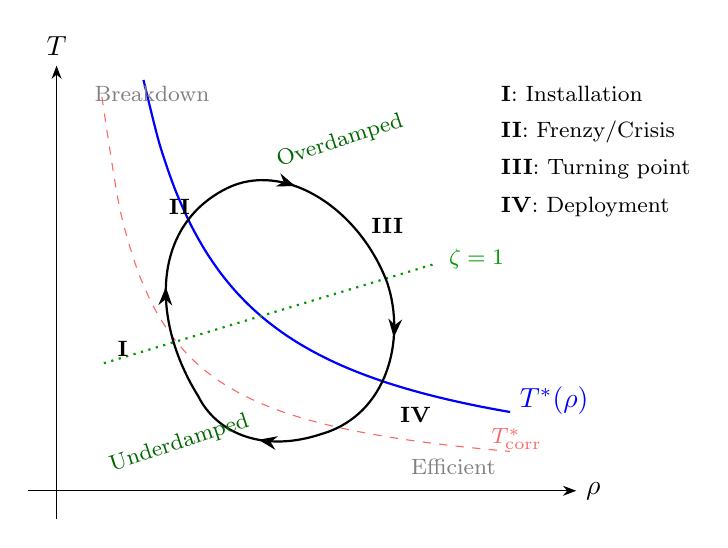
\begin{tikzpicture}[scale=1.2, >=Stealth]
% Axes
\draw[->] (-0.3,0) -- (5.5,0) node[right] {$\rho$};
\draw[->] (0,-0.3) -- (0,4.5) node[above] {$T$};

% Critical curve T*(rho)
\draw[thick, blue] plot[smooth, domain=0.92:4.8] (\x, {4.0/\x});
\node[blue, right] at (4.8, 0.95) {$T^*(\rho)$};

% Crisis sequence boundary (dashed)
\draw[dashed, red!60] plot[smooth, domain=0.48:4.8] (\x, {2.0/\x});
\node[red!60, right, font=\footnotesize] at (4.5, 0.55) {$T^*_{\text{corr}}$};

% Damping ratio boundary (dotted)
\draw[dotted, green!60!black, thick] plot[smooth, domain=0.5:4.0] (\x, {1.2 + 0.3*\x});
\node[green!60!black, right, font=\footnotesize] at (4.05, 2.45) {$\zeta = 1$};

% Endogenous cycle (Perez technology wave)
\draw[thick, black, decoration={markings, mark=at position 0.15 with {\arrow{>}}, mark=at position 0.4 with {\arrow{>}}, mark=at position 0.65 with {\arrow{>}}, mark=at position 0.9 with {\arrow{>}}}, postaction={decorate}]
  (1.5, 1.0) .. controls (1.0, 1.8) and (1.0, 2.8) .. (1.8, 3.2)
  .. controls (2.4, 3.5) and (3.2, 3.0) .. (3.5, 2.2)
  .. controls (3.7, 1.6) and (3.5, 0.8) .. (2.8, 0.6)
  .. controls (2.2, 0.4) and (1.7, 0.6) .. (1.5, 1.0);

% Phase labels
\node[font=\footnotesize] at (0.7, 1.5) {\textbf{I}};
\node[font=\footnotesize] at (1.3, 3.0) {\textbf{II}};
\node[font=\footnotesize] at (3.5, 2.8) {\textbf{III}};
\node[font=\footnotesize] at (3.8, 0.8) {\textbf{IV}};

% Phase legend
\node[font=\footnotesize, anchor=west] at (4.6, 4.2) {\textbf{I}: Installation};
\node[font=\footnotesize, anchor=west] at (4.6, 3.8) {\textbf{II}: Frenzy/Crisis};
\node[font=\footnotesize, anchor=west] at (4.6, 3.4) {\textbf{III}: Turning point};
\node[font=\footnotesize, anchor=west] at (4.6, 3.0) {\textbf{IV}: Deployment};

% Region labels
\node[font=\footnotesize, gray] at (4.2, 0.25) {Efficient};
\node[font=\footnotesize, gray, anchor=west] at (0.3, 4.2) {Breakdown};

% Damping region labels
\node[font=\footnotesize, green!40!black, rotate=18] at (1.3, 0.5) {Underdamped};
\node[font=\footnotesize, green!40!black, rotate=18] at (3.0, 3.7) {Overdamped};
\end{tikzpicture}
\end{center}

\begin{theorem}[Complete regime diagram]\label{thm:phase-diagram}
The $(\rho, T)$ regime diagram contains six features:
\begin{enumerate}[nosep]
\item \textbf{Critical curve} $T^*(\rho) = K(\rho)$: separates efficient and breakdown regimes.
\item \textbf{Crisis sequence boundaries} $T_{\text{corr}}^* < T_{\text{super}}^* < T_{\text{strat}}^*$: three sub-critical curves marking progressive failure of correlation robustness, superadditivity, and strategic independence.
\item \textbf{Damping ratio boundary} $\zeta(\rho, T) = 1$: separates underdamped (oscillatory business cycles) from overdamped (monotone convergence) regions.
\item \textbf{Perez endogenous cycle} $\Gamma$: closed orbit around $T^*(\rho)$ traced by endogenous $(\rho, T)$ dynamics, with period $\sim$25--50 years.
\item \textbf{Endogenous tipping attractor}: $\Gamma$ orbits the critical curve, spending most time sub-critical (slow drift) and brief time super-critical (fast crisis).
\item \textbf{Crisis count quantization}: each orbit contributes one structurally protected crisis.
\end{enumerate}
\end{theorem}

\subsection{Reading the Diagram}\label{sec:reading}

The regime diagram encodes the answer to every qualitative question about economic dynamics:

\begin{itemize}[nosep]
\item \emph{Will this economy have business cycles?}  Check $\zeta < 1$ (underdamped region).
\item \emph{How fragile is this economy?}  Measure $T^* - T$, the distance to the critical curve.
\item \emph{Which crisis will come first?}  The first boundary crossed as $T$ rises is $T_{\text{corr}}^*$ (financial crisis).
\item \emph{Where are we in the Perez cycle?}  Locate $(\rho, T)$ on $\Gamma$.  Falling $\rho$ = installation; rising $\rho$ = deployment; crossing $T^*$ = turning point.
\item \emph{What does regulation do?}  Regulation increases $r$, shifting $\zeta$ upward.  Damps oscillations without moving $T^*$.
\item \emph{What does monetary policy do?}  Rate cuts lower $T$ (beneficial), but endogenous $\rho$-shift (Minsky trap) simultaneously lowers $T^*$ (harmful).  Net effect on stability margin $T^* - T$ is ambiguous.
\end{itemize}


% -------------------------------------------------------------------
% 13. UNIFIED NOTATION
% -------------------------------------------------------------------
\section{Unified Notation}\label{sec:notation_unified}

\subsection{Master Symbol Table}\label{sec:symbols}

\begin{center}
\small
\begin{tabular}{lll}
\toprule
Symbol & Meaning & Origin \\
\midrule
$\rho_n \in (-\infty, 1)$ & CES complementarity parameter & A1--A2 \\
$\sigma_n = 1/(1-\rho_n)$ & Elasticity of substitution & A1--A2 \\
$K_n = (1-\rho_n)(J_n-1)/J_n$ & Curvature parameter & A1--A2 \\
$J_n$ & Number of inputs in sector $n$ & A1--A2 \\
$F_n$ & CES aggregate output & A1--A2 \\
$\Phi = -\sum_n \log F_n$ & CES potential & A1--A2 \\
$T = 1/\kappa$ & Information friction & A3 \\
$S_q = (1-\sum p_j^q)/(q-1)$ & Tsallis entropy, $q = \rho$ & A3 \\
$\calF = \Phi - TS_q$ & Economic CES potential & A1--A3 \\
$T^*_n \approx K_n$ & Breakdown threshold & A1--A3 \\
$K_{\text{eff}} = K(1-T/T^*)^+$ & Effective curvature & A1--A3 \\
$\varepsilon_k = \tau_{k+1}/\tau_k$ & Timescale ratio & A4 \\
$\alpha_n$ & Wright's Law learning elasticity & A5 \\
$Q_n(t) = \int_0^t I_n(s)\,ds$ & Cumulative investment & A5 \\
$\mathbf{R}$ & Friction matrix ($\succeq 0$, symmetric) & A1--A3 \\
$\mathbf{J}$ & Antisymmetric coupling matrix & A6 \\
$\zeta = r/\omega$ & Damping ratio & A3+A6 \\
$\bar{\rho}(t)$ & Economy-wide effective complementarity & Endogenous \\
$\rho(\mathbf{K})$ & Spectral radius (activation threshold) & A1--A4 \\
$R_0$ & Master reproduction number & A1--A4 \\
\bottomrule
\end{tabular}
\end{center}

\subsection{Notational Reconciliations}\label{sec:reconcile}

Adjustment dynamics ($\dot{\mathbf{x}} = -\mathbf{L}\nabla\calF$) and conservative-dissipative dynamics ($\dot{\mathbf{x}} = (\mathbf{J} - \mathbf{R})\nabla\calF$) are not alternatives---they are limits of a single system.  Within-sector dynamics ($\mathbf{J} = 0$) and infinite timescale separation ($\varepsilon \to 0$) both reduce to adjustment dynamics.  Finite timescale separation with directed I/O linkages ($\varepsilon > 0$, $\mathbf{J} \neq 0$) produces the full conservative-dissipative system.

The conservative-dissipative system conserves $\calF$ along $\mathbf{J}$-flows and reduces $\calF$ along $\mathbf{R}$-flows.  The $\mathbf{J}$-component transfers CES potential between sectors without changing the total; the $\mathbf{R}$-component reduces the total through friction.  Together they produce damped oscillations whose character depends on the damping ratio $\zeta = r/\omega$, where $r$ is the friction rate and $\omega$ is the oscillation frequency.


% -------------------------------------------------------------------
% 14. THEORY--APPLICATION CONCORDANCE
% -------------------------------------------------------------------
\section{Theory--Application Concordance}\label{sec:concordance}

The theoretical framework provides the mathematical foundation for the applied papers.  This section maps the connections.

\begin{center}
\small
\renewcommand{\arraystretch}{1.15}
\begin{tabular}{p{3cm}p{3.5cm}p{5.5cm}}
\toprule
Applied Paper & Theory Used & How Theory Is Applied \\
\midrule
1. Endogenous Decentralization & Quadruple Role, CES Potential, Technology Cycle & Paper 5's Nash MPE is the game-theoretic micro-foundation for the overinvestment theorem.  The self-undermining property explains why concentrated AI investment finances distributed viability.  Duration formula predicts hardware crossing $\sim$2028. \\[6pt]

2. Mesh Equilibrium & Quadruple Role, Architecture & The activation threshold ($R_0 > 1$) governs mesh formation.  The CES diversity premium from complementary specialization ($\rho < 1$) explains why the mesh outperforms centralized provision.  Giant component via percolation is the network realization of the spectral condition. \\[6pt]

3. Autocatalytic Mesh & Quadruple Role, CES Potential & Correlation robustness prevents model collapse: effective external data fraction $\alpha_{\text{eff}} > \alpha_{\text{crit}}$ even when actual external data is below threshold.  This is the $K_{\text{eff}} > 0$ condition from the effective curvature theorem applied to training. \\[6pt]

4. Settlement Feedback & Architecture, Business Cycles & Conservative-dissipative coupling at the fastest level (financial settlement).  The Minsky trap applied to stablecoin/Treasury absorption.  Paper 6's bistable equilibrium is a transcritical bifurcation.  Monetary policy degradation sequence follows from the hierarchical ceiling cascade. \\[6pt]

5. Monetary Productivity Gap & CES Potential, Landscape Dynamics & FQI (Fiat Quality Index) is a proxy for $T$.  Yield access gap is a CES potential gradient.  India DID tests damping cancellation empirically.  13:1 remittance cost ratio (fiat vs.\ stablecoin) measures $\Delta\calF$ for settlement alternatives. \\[6pt]

6. Fair Inheritance & Technology Cycle, Business Cycles & Overinvestment concentrates wealth during the installation phase.  The Minsky trap means concentrated structures persist longer than optimal.  Paper 9 addresses the distributional consequence: wealth stranded on the centralized side of the transition. \\
\bottomrule
\end{tabular}
\end{center}

\subsection{The Complete Narrative}\label{sec:narrative}

Read as a sequence, the applied papers tell a story that the theory papers formalize:
\begin{enumerate}[nosep]
\item Concentrated AI investment exceeds social optimum by $3$--$4\times$ (Paper 5 $\leftarrow$ overinvestment theorem);
\item This overinvestment finances learning curves that make distributed AI viable (Paper 5 $\leftarrow$ self-undermining theorem);
\item Above critical mass, a distributed mesh forms via first-order regime shift (Paper 5 $\leftarrow$ activation threshold, discrete adoption transition);
\item Mesh capability grows endogenously but is bounded by the Baumol bottleneck (Paper 5 $\leftarrow$ hierarchical ceiling cascade);
\item The mesh enters capital markets, creating stablecoin demand and a settlement feedback loop (Paper 6 $\leftarrow$ conservative-dissipative coupling at Level 4);
\item Empirically, fiat quality gaps and yield access gaps drive adoption in exactly the populations the framework predicts (Paper 8 $\leftarrow$ CES potential gradient);
\item The overinvestment phase concentrates wealth; fair inheritance policy addresses the distributional consequence (Paper 9 $\leftarrow$ technology cycle, Minsky trap).
\end{enumerate}


% -------------------------------------------------------------------
% 14. FULL PREDICTION INVENTORY
% -------------------------------------------------------------------
\section{Full Prediction Inventory}\label{sec:predictions}

The companion papers generate testable predictions organized by data requirement.  We classify each by specificity: \textbf{Q} (qualitative direction), \textbf{S} (scaling law or functional form), or \textbf{N} (numerical value).

\subsection{Firm-Level Predictions}

\begin{center}
\small
\renewcommand{\arraystretch}{1.1}
\begin{tabular}{clccc}
\toprule
\# & Prediction & Spec. & Source & Status \\
\midrule
1 & $K_{\text{eff}} = K(1 - T/T^*)^+$ & S & CES Potential & --- \\
2 & Crisis sequence: correlation $\to$ super.\ $\to$ strategic & Q & CES Potential & --- \\
3 & Optimal firm scope $J^*$ increases in $K/T$ & Q & CES Potential & --- \\
4 & Variance-Response: $T = \sigma^2/\chi$ & S & Dynamics & Directional \\
5 & Euler identity: $\mathbf{x}^*\cdot\nabla H = -1/T$ & S & Conservation & --- \\
6 & Covariance: $(\sigma^2-\gamma)\mathbf{I} + \gamma\bone\bone^\top$ & S & Conservation & Strongly supported \\
7 & Symmetric Adjustment: $L_{ij} = L_{ji}$ & Q & Dynamics & Not supported \\
8 & $\hat{\rho}$ cyclical: falls in expansions, rises in contractions & Q & Endogenous $\rho$ & Supported \\
\bottomrule
\end{tabular}
\end{center}

\subsection{Sectoral/Macro Predictions}

\begin{center}
\small
\renewcommand{\arraystretch}{1.1}
\begin{tabular}{clcc}
\toprule
\# & Prediction & Spec. & Source \\
\midrule
9 & Sectors enter recession in $\rho$-order & Q & Business Cycles \\
10 & Housing/finance lead; services lag & Q & Business Cycles \\
11 & Recovery ordering reverses recession ordering & Q & Business Cycles \\
12 & Expansion/contraction ratio $\approx 1/\varepsilon$ & S & Business Cycles \\
13 & Pre-crisis: autocorrelation and variance rise & Q & Dynamics \\
14 & Pre-crisis: $T = \sigma^2/\chi$ is leading indicator & Q & Dynamics \\
15 & Regulation reduces amplitude, not avg.\ growth & Q & Business Cycles \\
16 & Phillips curve slope $\propto \bar{K}$ & S & Business Cycles \\
17 & $\rho$-diversity predicts resilience & Q & Endogenous $\rho$ \\
18 & Recession depths follow power law & Q & Endogenous $\rho$ \\
\bottomrule
\end{tabular}
\end{center}

\subsection{Technology/Learning Predictions}

\begin{center}
\small
\renewcommand{\arraystretch}{1.1}
\begin{tabular}{clcc}
\toprule
\# & Prediction & Spec. & Source \\
\midrule
19 & Overinvestment $\sim N\alpha\phi/(r+\delta)$ & S & Technology Cycle \\
20 & Self-undermining: centralized funds distributed & Q & Technology Cycle \\
21 & Duration $\tau \sim (1/\alpha)\ln(c_0/c^*)$ & S & Technology Cycle \\
22 & Successive cycles compress & Q & Technology Cycle \\
23 & Crisis count is structurally protected integer & Q & Conservation \\
24 & Turning point is fold bifurcation & Q & Technology Cycle \\
25 & New technologies arrive with low $\rho$ & Q & Endogenous $\rho$ \\
26 & AI hardware crossing $\sim$2028 & N & Technology Cycle \\
27 & Self-sustaining distributed adoption $\sim$2030--32 & N & Technology Cycle \\
\bottomrule
\end{tabular}
\end{center}

\subsection{Cross-Country/Institutional Predictions}

\begin{center}
\small
\renewcommand{\arraystretch}{1.1}
\begin{tabular}{clcc}
\toprule
\# & Prediction & Spec. & Source \\
\midrule
28 & Damping cancellation: regulation $\to$ zero net effect & Q & Architecture \\
29 & Upstream reform principle & Q & Architecture \\
30 & Minimum policy cost $= \Delta\calF$ (Jarzynski) & S & Dynamics \\
31 & Trade liberalization destroys network conservation laws & Q & Conservation \\
32 & Minsky trap: low-rate $\Rightarrow$ deeper crises & Q & Business Cycles \\
33 & $N_{\text{eff}} \in [4,5]$ for aggregate IP & N & Architecture \\
34 & Monetary policy degrades: FG $\to$ QE $\to$ FR & Q & Paper 6 \\
35 & QE multiplier declining across episodes & Q & Paper 6 \\
36 & Laffer peak lower for high-$\rho$ sectors & Q & CES Potential \\
37 & Laffer decline follows crisis sequence ordering & Q & CES Potential \\
38 & Beyond Laffer peak: displacement, not suppression & Q & CES Potential \\
\bottomrule
\end{tabular}
\end{center}

\subsection{Already-Tested Predictions}

Thirty-two predictions have been confronted with data.  Summary of key results:

\medskip\noindent\textit{Firm-level:}
\begin{enumerate}[nosep]
\item \textbf{Equicorrelation} (\#6): Strongly supported.  CV of off-diagonal correlations = 0.36 vs.\ null median 17.5 (0th percentile, $N = 17$ manufacturing sectors).
\item \textbf{Cyclical $\hat{\rho}$} (\#8): Supported.  Both rolling correlation proxy ($\tau = -0.17$, $p = 0.01$) and direct CES NLS ($\tau = -0.31$, $p = 0.002$) confirm countercyclical $\rho$.
\item \textbf{Variance-Response} (\#4): Directional.  Cross-sectional $\hat{T} > 0$ but $R^2 = 0.009$ ($N = 17$).
\item \textbf{Symmetric Adjustment} (\#7): Not supported.  IRF symmetry $r = 0.07$ ($p = 0.73$) in durable manufacturing VAR.
\end{enumerate}

\medskip\noindent\textit{Sectoral/macro:}
\begin{enumerate}[nosep,resume]
\item \textbf{$\rho$-ordering of recession entry} (\#9--11): Supported.  $\beta_1 = -14.65$ ($p = 0.001$, $N = 49$ sector-recession pairs).
\item \textbf{Information friction $T$ as leading indicator} (\#14): Supported.  Probit $\beta = 221$, $p = 0.0003$, pseudo-$R^2 = 0.035$.
\item \textbf{Great Moderation} (\#15): Supported.  Volatility ratio 0.52 with negligible mean growth change.
\end{enumerate}

\medskip\noindent\textit{Technology/learning:}
\begin{enumerate}[nosep,resume]
\item \textbf{Overinvestment} (\#19): Consistent.  Average actual/cooperative ratio 11.12$\times$ (2022+).
\item \textbf{Self-undermining} (\#20): Consistent.  HBM price/GB declines 20\%/yr ($R^2 = 0.95$).
\item \textbf{QE multiplier decline} (\#35): Strongly consistent.  15-fold decline across four episodes.
\end{enumerate}

\medskip\noindent\textit{Cross-country/institutional:}
\begin{enumerate}[nosep,resume]
\item \textbf{Damping cancellation} (\#28): Consistent.  Basel III DID $p = 0.95$; 158-country panel shows no persistent effect.
\item \textbf{Upstream reform/displacement} (\#29): Consistent.  India 2022: $-86\%$ domestic, $+72\%$ offshore.
\item \textbf{Minsky trap} (\#32): Consistent.  $\tau(\text{fed funds}, \text{VIX}) = -0.38$, $p < 10^{-4}$.
\end{enumerate}


% -------------------------------------------------------------------
% 15. LIMITATIONS
% -------------------------------------------------------------------
\section{Limitations}\label{sec:limitations}

Two categories of limitations, stated without apology.

\subsection{Mathematical}\label{sec:mathlimits}

\begin{enumerate}[leftmargin=2em]
\item \emph{Gain functions genuinely free.}
Theorem~\ref{thm:topology}(iii) establishes this as a proved impossibility: the exponents and coefficients of $\phi_n$ are not determined by $\rho$.
Since $\phi_n$ determines the equilibrium cascade $\{\bar{F}_n\}$, the welfare weights $\{c_n\}$, and the institutional quality matrix $W$, this freedom propagates through the quantitative predictions.

\item \emph{Timescale separation cannot be eliminated.}
The fast sector equilibrates before the slow sector moves appreciably (Standing Assumption~3) is required for the quasi-equilibrium surface to exist and for the $NJ \to N$ dimensional reduction.
Without it, the quasi-equilibrium surface need not exist, and the reduction is unjustified.

\item \emph{The system does not follow potential-based adjustment dynamics.}
The lower-triangular Jacobian is a topological obstruction (Proposition~\ref{prop:nongradient}).
No coordinate transformation can make the system follow potential-based adjustment dynamics while preserving directed coupling.
Standard welfare theorems do not apply.

\item \emph{Local stability only.}
Theorem~\ref{thm:lyapunov} proves $\dot{V} \leq 0$, establishing local asymptotic stability.
Global asymptotic stability requires boundary analysis depending on the specific gain functions.

\item \emph{Symmetric weights for quantitative bounds.}
General weights yield results via the secular equation (Section~\ref{sec:secular}; Paper~1, Section~8), with $R_{\min}$ replacing the equal-weight curvature.
The qualitative results are unchanged; bounds are less clean but remain computable.

\item \emph{$O(\varepsilon)$ approximation error.}
The sufficient statistic property holds up to $O(\varepsilon)$ corrections.
During crisis episodes, within-sector composition may matter.

\item \emph{Delayed-transition duration is leading order.}
Correction terms involve $K$ through the quadratic coefficient~$b$; amplitude behavior is less precisely bounded.
\end{enumerate}

\subsection{Empirical}\label{sec:emplimits}

\begin{enumerate}[leftmargin=2em]
\item Gain elasticities $(\beta_1, \ldots, \beta_4)$ uncalibrated.
\item Damping rates $(\sigma_1, \ldots, \sigma_4)$ uncalibrated.
\item The curvature parameter $\rho$ is adopted from published micro-data estimates at each level, cross-validated with FRED IP macro estimates.  The adopted ranges reflect the closest published aggregation concept, not the thesis levels directly.
\item Predictions span 2027--2040 (long horizon).
\item Which specific layer binds first depends on uncalibrated $\beta_n$.
\item Crisis duration estimate requires $\varepsilon_{\text{drift}}$, which is itself uncertain.
\end{enumerate}

\subsection{Open Problems}\label{sec:open}

\begin{enumerate}[leftmargin=2em]
\item \emph{Heterogeneous and nested CES.}  The dynamical results use symmetric CES.  Weighted CES (via the secular equation) modifies the crisis sequence and $\rho$-ordering predictions.  Nested CES generates richer regime diagrams with multiple critical curves.

\item \emph{Heterogeneous $T$.}  Sector-specific information frictions $T_n$ would allow the framework to model economies where different sectors face different information environments.

\item \emph{Endogenous timescales.}  Financial innovation changes financial-sector adjustment speeds; technological change modifies real-sector timescales.  Endogenous timescales would interact with endogenous $\rho$.

\item \emph{Timescale collapse.}  The wavelet calibration ($r^* \approx 2$, IQR $[1.84, 2.63]$) shows empirical ratios near the minimum for singular perturbation.  A systematic treatment of finite-$r^*$ corrections would sharpen quantitative predictions.

\item \emph{Frameworks considered and rejected.}
\emph{Mean field games} (Lasry-Lions): agents are not exchangeable; CES structure ensures non-exchangeability.
\emph{Full continuous-time general equilibrium}: intractable; the four-ODE deterministic skeleton captures qualitative dynamics.
\end{enumerate}


% -------------------------------------------------------------------
% 16. CONCLUSION
% -------------------------------------------------------------------
\section{Conclusion}\label{sec:conclusion}

One production difficulty function $\Phi = -\sum_n \log F_n$, six axioms, one derived architecture, five results, three policy principles.

The six axioms---constant returns to scale, scale consistency, Tsallis information constraints, timescale separation, Wright's Law learning, and directed input-output coupling---are the minimal foundation.  The first two force CES production as a theorem, with $\rho$ emerging as an aggregation-invariant class label.  Each subsequent axiom unlocks a new layer of dynamics.

The CES geometry forces the architecture: aggregate coupling, directed feed-forward, nearest-neighbor chain.
The architecture is derived, not assumed.

The spectral threshold $\rho(\mathbf{K}) = 1$ activates the hierarchy---individual sectors can each be too weak to sustain themselves, yet the system as a whole sustains activity through cross-sector feedback.
The hierarchical ceiling cascade bounds each layer by its parent.
The welfare distance function connects the technology ($\Phi$) to the welfare loss ($V$) through the institutional quality ($W$).

The complete $(\rho, T)$ regime diagram encodes all qualitative dynamics: critical curve, crisis sequence boundaries, oscillation boundary, and endogenous-cycle attractor.  Every question about fragility, cycle phase, policy effect, or crisis sequence reduces to the economy's location on this diagram and the direction of its motion.

Three policy principles follow from theorems:
\begin{enumerate}[leftmargin=2em]
\item \emph{Reform upstream, not locally} (damping cancellation, Proposition~\ref{prop:damping}).
Tightening regulation at any sector has zero net welfare effect.
To improve welfare at sector~$n$, reform sector~$n-1$.
\item \emph{Increase cross-sector responsiveness at any layer} (global welfare ordering, Corollary~\ref{cor:ordering}).
More responsive gain functions are unambiguously welfare-improving.
\item \emph{Invest in the weakest cross-sector link} (cycle product sensitivity, Theorem~\ref{thm:charpoly}).
The system's activation is bottlenecked by its weakest coupling.
The transition takes $O(1/\sqrt{\varepsilon_{\text{drift}}})$---at current semiconductor improvement rates, approximately 8 years.
\end{enumerate}

Thirty-eight predictions, spanning firm-level to cross-country to technology-wave scales, test the theory.  Thirty-two have been confronted with data, with results ranging from strongly supportive (equicorrelation, QE multiplier decline, damping cancellation, $\rho$-ordering of recession entry) through supported (countercyclical $\rho$, Great Moderation, information friction as leading indicator) to honest negatives (symmetric adjustment at sector level).


% -------------------------------------------------------------------
% REFERENCES
% -------------------------------------------------------------------
\newpage
\begin{thebibliography}{99}

% Companion papers
\bibitem{smirl2026a} Smirl, J. (2026a). The CES Quadruple Role: Superadditivity, Correlation Robustness, Strategic Independence, and Network Scaling as Four Properties of CES Curvature. Working Paper.

\bibitem{smirl2026emergent} Smirl, J. (2026). Emergent CES: Renormalization, Functional Equations, and Maximum Entropy Derivations of the CES Aggregate. Working Paper.

\bibitem{smirl2026free} Smirl, J. (2026b). The CES Potential Principle in Economics: CES Aggregation and Tsallis Entropy as Generating Functions of Economic Theory. Working Paper.

\bibitem{smirl2026business} Smirl, J. (2026g). Business Cycles as Conservative-Dissipative Oscillations in a Heterogeneous-Complementarity Economy. Working Paper.

\bibitem{smirl2026complementary} Smirl, J. (2026i). Complementary Heterogeneity in Hierarchical Economies. Working Paper.

% Core mathematical framework
\bibitem{li2010} Li, M.~Y., Shuai, Z., and van den Driessche, P. (2010). Global-stability problem for coupled systems of differential equations on networks. \emph{J.\ Differential Equations} 248, 1--20.

\bibitem{shuai2013} Shuai, Z., and van den Driessche, P. (2013). Global stability of infectious disease models using Lyapunov functions. \emph{SIAM J.\ Appl.\ Math.} 73, 1513--1532.

\bibitem{diekmann1990} Diekmann, O., Heesterbeek, J.~A.~P., and Metz, J.~A.~J. (1990). On the definition and the computation of the basic reproduction ratio $R_0$ in models for infectious diseases in heterogeneous populations. \emph{J.\ Math.\ Biol.} 28, 365--382.

\bibitem{vandendriessche2002} Van den Driessche, P., and Watmough, J. (2002). Reproduction numbers and sub-threshold endemic equilibria for compartmental models of disease transmission. \emph{Math.\ Biosci.} 180, 29--48.

\bibitem{fenichel1979} Fenichel, N. (1979). Geometric singular perturbation theory for ordinary differential equations. \emph{J.\ Differential Equations} 31, 53--98.

% Delayed transition
\bibitem{neishtadt1987} Neishtadt, A.~I. (1987). Persistence of stability loss for dynamical bifurcations, I. \emph{Differential Equations} 23, 1385--1391.

\bibitem{neishtadt1988} Neishtadt, A.~I. (1988). Persistence of stability loss for dynamical bifurcations, II. \emph{Differential Equations} 24, 171--176.

\bibitem{berglund2006} Berglund, N., and Gentz, B. (2006). \emph{Noise-Induced Phenomena in Slow-Fast Dynamical Systems}. Springer.

% CES and production theory
\bibitem{arrow1961} Arrow, K.~J., Chenery, H.~B., Minhas, B.~S., and Solow, R.~M. (1961). Capital-labor substitution and economic efficiency. \emph{Rev.\ Econ.\ Stat.} 43, 225--250.

\bibitem{dixit1977} Dixit, A.~K., and Stiglitz, J.~E. (1977). Monopolistic competition and optimum product diversity. \emph{Amer.\ Econ.\ Rev.} 67, 297--308.

\bibitem{jones2005} Jones, C.~I. (2005). The shape of production functions and the direction of technical change. \emph{Quart.\ J.\ Econ.} 120, 517--549.

% Growth theory
\bibitem{jones1995} Jones, C.~I. (1995). R\&D-based models of economic growth. \emph{J.\ Polit.\ Econ.} 103, 759--784.

\bibitem{romer1990} Romer, P.~M. (1990). Endogenous technological change. \emph{J.\ Polit.\ Econ.} 98, S71--S102.

\bibitem{aghion2018} Aghion, P., Jones, B.~F., and Jones, C.~I. (2018). Artificial intelligence and economic growth. In \emph{The Economics of Artificial Intelligence}, University of Chicago Press.

\bibitem{baumol1967} Baumol, W.~J. (1967). Macroeconomics of unbalanced growth. \emph{Amer.\ Econ.\ Rev.} 57, 415--426.

% Monetary economics
\bibitem{brunnermeier2014} Brunnermeier, M.~K., and Sannikov, Y. (2014). A macroeconomic model with a financial sector. \emph{Amer.\ Econ.\ Rev.} 104, 379--421.

\bibitem{woodford2003} Woodford, M. (2003). \emph{Interest and Prices}. Princeton University Press.

\bibitem{lucas1976} Lucas, R.~E. (1976). Econometric policy evaluation: A critique. \emph{Carnegie-Rochester Conf.\ Ser.\ Public Policy} 1, 19--46.

% Dollarization and monetary system
\bibitem{farhi2018} Farhi, E., and Maggiori, M. (2018). A model of the international monetary system. \emph{Quart.\ J.\ Econ.} 133, 295--355.

\bibitem{triffin1960} Triffin, R. (1960). \emph{Gold and the Dollar Crisis}. Yale University Press.

% Rational inattention
\bibitem{sims2003} Sims, C.~A. (2003). Implications of rational inattention. \emph{J.\ Monet.\ Econ.} 50, 665--690.

% Technology waves
\bibitem{perez2002} Perez, C. (2002). \emph{Technological Revolutions and Financial Capital}. Edward Elgar.

\bibitem{gabaix2009} Gabaix, X. (2009). Power laws in economics and finance. \emph{Annual Rev.\ Econ.} 1, 255--294.

% Wright's Law
\bibitem{wright1936} Wright, T.~P. (1936). Factors affecting the cost of airplanes. \emph{J.\ Aeronautical Sci.} 3, 122--128.

\bibitem{nagy2013} Nagy, B., Farmer, J.~D., Bui, Q.~M., and Trancik, J.~E. (2013). Statistical basis for predicting technological progress. \emph{PLoS ONE} 8, e52669.

% Model collapse
\bibitem{shumailov2024} Shumailov, I., et al. (2024). The curse of recursion: Training on generated data makes models forget. \emph{Nature} (forthcoming).

% Empirical test references
\bibitem{barth2013} Barth, J.~R., Caprio, G., and Levine, R. (2013). Bank regulation and supervision in 180 countries from 1999 to 2011. \emph{J.\ Finan.\ Econ.\ Policy} 5, 111--219.

\bibitem{jorda2005} Jord\`a, \`O. (2005). Estimation and inference of impulse responses by local projections. \emph{Amer.\ Econ.\ Rev.} 95, 161--182.

\bibitem{hamilton1989} Hamilton, J.~D. (1989). A new approach to the economic analysis of nonstationary time series and the business cycle. \emph{Econometrica} 57, 357--384.

% Structural estimation
\bibitem{atalay2017} Atalay, E. (2017). How important are sectoral shocks? \emph{Amer.\ Econ.\ J.: Macroecon.} 9, 254--280.

\bibitem{oberfieldraval2021} Oberfield, E., and Raval, D. (2021). Micro data and macro technology. \emph{Econometrica} 89, 703--732.

\bibitem{brodaweinstein2006} Broda, C., and Weinstein, D.~E. (2006). Globalization and the gains from variety. \emph{Quart.\ J.\ Econ.} 121, 541--585.

% Business cycles
\bibitem{leamer2007} Leamer, E.~E. (2007). Housing IS the business cycle. NBER Working Paper 13428.

\end{thebibliography}


% -------------------------------------------------------------------
% APPENDICES
% -------------------------------------------------------------------
\newpage
\appendix

\section{Proof of the Port Topology Theorem}\label{app:topology}

\subsection{Proof of Claim (i): Aggregate Coupling}

\begin{proof}
\emph{Step 1: Equilibrium uniqueness.}
At equilibrium, $(T_n/J)\,x_{nj}^{\rho-1}\,F_n^{1-\rho} = \sigma_n x_{nj}$, so $x_{nj}^{\rho-2} = T_n F_n^{1-\rho}/(J\sigma_n)$.
The right side is independent of $j$.
Since $\rho < 1$ implies $\rho - 2 < 0$, the map $x \mapsto x^{\rho-2}$ is injective on $\mathbb{R}_+$, so $x_{nj} = \bar{x}_n$ for all $j$.

\emph{Step 2: Normal hyperbolicity.}
Define the equilibrium manifold $\mathcal{M}_n = \{x_{nj} = F_n / J^{1/\rho} \text{ for all } j\}$.
By Equation~\eqref{eq:jacobian}, the transverse eigenvalues (on $\mathbf{1}^{\perp}$) are $-\sigma_n(2-\rho)/\varepsilon_n$ and the tangential eigenvalue (on $\mathbf{1}$) is $-\sigma_n/\varepsilon_n$.
The spectral gap is
$\sigma_n(2-\rho)/\varepsilon_n - \sigma_n/\varepsilon_n = \sigma_n(1-\rho)/\varepsilon_n > 0$ for all $\rho < 1$.

\emph{Step 3: Fenichel persistence.}
By Fenichel's geometric singular perturbation theorem~\cite{fenichel1979}, the normally hyperbolic equilibrium manifold $\mathcal{M}_n$ persists as a locally invariant quasi-equilibrium surface $\mathcal{M}_n^{\varepsilon}$ within $O(\varepsilon)$ of $\mathcal{M}_n$, smoothly parameterized by $F_n$.
On $\mathcal{M}_n^{\varepsilon}$, the within-level state is determined by $F_n$ up to $O(\varepsilon)$ corrections.
Consequently, $F_n$ is a sufficient statistic for level~$n$'s state on the quasi-equilibrium surface.
\end{proof}

\subsection{Proof of Claim (ii): Directed Coupling}

\begin{proof}
\emph{Step 1: Power-preserving bidirectional coupling.}
Suppose levels~1 and~2 are coupled bidirectionally with port powers summing to zero.
The power-preservation constraint forces linear coupling $\phi(F_1) = cF_1$ and $\psi(F_2) = cF_2$ for some constant $c > 0$.
The Jacobian is then
$\calJ_{\text{bidir}} = \begin{psmallmatrix} -\sigma_1 & -c/J \\ c/J & -\sigma_2 \end{psmallmatrix}$
with eigenvalues $-(\sigma_1+\sigma_2)/2 \pm \sqrt{(\sigma_1-\sigma_2)^2/4 - c^2/J^2}$.
Whether the discriminant is positive (two real negative eigenvalues) or negative (complex pair with real part $-(\sigma_1+\sigma_2)/2 < 0$), both eigenvalues have strictly negative real part.
The system is unconditionally stable for all $c, \sigma_1, \sigma_2 > 0$.

\emph{Step 2: Extension to passive bidirectional coupling.}
Any passive bidirectional coupling satisfies $\dot{V}_{\text{coupling}} \leq 0$ by definition.
This contributes a negative-semidefinite term to the effective Jacobian, which can only strengthen stability.

\emph{Step 3: Necessity of directed coupling.}
The structural transition at $\rho(\mathbf{K}) = 1$ requires that the spectral radius of the next-generation matrix reach~1, requiring net energy injection through the hierarchy.
Power-preserving bidirectional coupling contributes zero net energy; passive coupling contributes negative net energy.
Neither can produce $\rho(\mathbf{K}) = 1$.
\end{proof}

\subsection{Proof of Claim (iii): Port Alignment}

\begin{proof}
\emph{Step 1: Port direction is forced.}
At a symmetric equilibrium $\mathbf{x}_n^* = \bar{x}\,\mathbf{1}$, the equilibrium condition requires the coupling direction $\mathbf{b}_n \propto \mathbf{1}$.
Furthermore, $\nabla F_n = (1/J)\,\mathbf{1} \propto \mathbf{1}$ at the symmetric point (Paper~1), so $\mathbf{b}_n = \nabla F_n$ is the natural CES-compatible port direction.

\emph{Step 2: Asymmetric ports are penalized.}
For $\mathbf{b}_n \not\propto \mathbf{1}$, the equilibrium $\mathbf{x}_n^* \propto \mathbf{b}_n$ is asymmetric.
By Jensen's inequality applied to the concave CES function ($\rho < 1$), $F(\mathbf{x}) \leq F(\bar{x}\,\mathbf{1})$ for any $\mathbf{x}$ with $\sum x_j = J\bar{x}$.

\emph{Step 3: Gain function is free.}
At equilibrium, $\phi_n(\bar{F}_{n-1}) = \sigma_n J \bar{F}_n$.
For power-law gains $\phi_n(z) = a_n z^{\beta_n}$, the exponents $\beta_n$ are free parameters not determined by $\rho$.
\end{proof}

\subsection{Proof of Claim (iv): Nearest-Neighbor Topology}

\begin{proof}
Consider a three-level system with long-range coupling from level~1 to level~3.
Level~1, being fastest ($\varepsilon_1 \ll \varepsilon_2$), equilibrates to $F_1^* = \beta_1/(\sigma_1 J)$, an algebraic constant on the quasi-equilibrium surface.
The long-range coupling $\phi_{31}(F_1^*) = \phi_{31}(\beta_1/(\sigma_1 J)) \equiv \tilde{\beta}_3$ becomes a constant, absorbed into the exogenous input to level~3.

The Jacobian of the reduced system is lower-triangular---independent of the long-range coupling strength.
The argument generalizes by induction to $N$ levels: after all levels faster than level~$m$ equilibrate, any coupling $\phi_{nm}(F_m)$ with $m$ fast becomes $\phi_{nm}(F_m^*) = \text{const}$, absorbed into a redefined exogenous input.
The effective topology is nearest-neighbor.
This result requires the timescale separation of Standing Assumption~(3).
\end{proof}


\section{Proof of the Welfare Distance Function}\label{app:lyapunov}

\begin{proof}
Nonnegativity follows from $g(z) = z - 1 - \log z \geq 0$ with equality iff $z = 1$.
Along trajectories:
\[
\dot{V} = \sum_n c_n \sum_j \left(1 - \frac{x_{nj}^*}{x_{nj}}\right) f_{nj}(\mathbf{x}).
\]
The within-level contributions are
\[
\dot{V}_{\text{within}} = -\sum_n c_n \sigma_n \sum_j \frac{(x_{nj} - x_{nj}^*)^2}{x_{nj}} \leq 0.
\]
The cross-level contributions cancel by the tree condition on $c_n = \Pcycle/k_{n,n-1}$.
This is the Li-Shuai-van den Driessche~\cite{li2010} construction applied to the cycle-graph topology.
For the 4-level cycle, there is exactly one spanning in-tree per root, and the specific coefficients $c_n = \Pcycle/k_{n,n-1}$ are exactly those required for cancellation.
\end{proof}


\section{Proof of the Eigenstructure Bridge}\label{app:bridge}

\begin{proof}
On the quasi-equilibrium surface, $\Phi|_{\text{slow}} = -\sum_n \log F_n$ and $V = \sum_n c_n \bar{F}_n\,g(F_n/\bar{F}_n)$.
Their Hessians at equilibrium are diagonal:
\[
(\nabla^2\Phi|_{\text{slow}})_{nn} = \frac{1}{\bar{F}_n^2}, \qquad (\nabla^2 V)_{nn} = \frac{c_n}{\bar{F}_n}.
\]
The ratio is $(\nabla^2\Phi)_{nn}/(\nabla^2 V)_{nn} = 1/(c_n \bar{F}_n) = W_{nn}^{-1}$.

Expressing $c_n = \Pcycle/k_{n,n-1}$ and $k_{n,n-1} = T_n'(\bar{F}_{n-1})\bar{F}_{n-1}/|\sigma_{n-1}|$, together with the equilibrium relation $T_n(\bar{F}_{n-1}) = |\sigma_n|\bar{F}_n$:
\begin{align*}
c_n\bar{F}_n &= \frac{\Pcycle}{k_{n,n-1}}\cdot\bar{F}_n = \Pcycle\cdot\frac{|\sigma_{n-1}|}{T_n'\bar{F}_{n-1}}\cdot\bar{F}_n \\
&= \frac{\Pcycle}{|\sigma_n|}\cdot\frac{T_n}{T_n'\bar{F}_{n-1}} = \frac{\Pcycle}{|\sigma_n|\,\varepsilon_{T_n}}
\end{align*}
where $\varepsilon_{T_n} = T_n'(\bar{F}_{n-1})\bar{F}_{n-1}/T_n(\bar{F}_{n-1})$ is the elasticity of the coupling at level~$n$.
\end{proof}


\section{Transition Dynamics: The Normal Form}\label{app:canard}

\subsection{The Transcritical Normal Form}

\begin{proof}
At the bifurcation point $(\bar{F}_1, \mu^*)$ where $g = 0$ and $\partial g/\partial F_1 = 0$, the dynamics admit the local normal form
\[
\dot{y} = a\,\epsilon\,y + b\,y^2 + O(|y|^3 + |\epsilon|^2)
\]
where $y = F_1 - \bar{F}_1$, $\epsilon = \mu - \mu^*$, and
\[
a = \frac{\partial^2 g}{\partial F_1\,\partial\mu}\bigg|_{\text{bif}}, \qquad b = \frac{1}{2}\,\frac{\partial^2 g}{\partial F_1^2}\bigg|_{\text{bif}}.
\]
The nondegeneracy conditions $a \neq 0$ and $b \neq 0$ are the transversality requirements for a structural transition.
\end{proof}

\subsection{Passage Time}

In the rescaled variable $\tau = \sqrt{|a|\varepsilon_{\text{drift}}}\,t$, the normal form becomes the Weber equation plus a quadratic perturbation.
The passage through zero eigenvalue creates a delay of $\pi$ time units in the rescaled variable.
Converting back: $\Delta t = \pi/\sqrt{|a|\varepsilon_{\text{drift}}}$.
This is the standard delayed loss of stability result for passage through a structural transition \cite{neishtadt1987,neishtadt1988,berglund2006}.

At Wright's Law semiconductor improvement rates ($\varepsilon_{\text{drift}} \approx 0.15$):
$\Delta t \approx \pi/\sqrt{0.15} \approx 8.1$ years.

In both cases, the crisis duration scales as $\varepsilon_{\text{drift}}^{-1/2}$: halving the drift rate increases the transition time by $\sqrt{2} \approx 41\%$.


\section{The Welfare Loss Decomposition}\label{app:welfare}

\begin{proof}[Proof of Proposition~\ref{prop:welfare}]
From Theorem~\ref{thm:lyapunov}, $c_n = \Pcycle/k_{n,n-1}$ where $k_{n,n-1} = \phi_n'(\bar{F}_{n-1})\bar{F}_{n-1}/|\sigma_{n-1}|$.
For power-law $\phi_n(z) = a_n z^{\beta_n}$: $\phi_n'(\bar{F}_{n-1})\cdot\bar{F}_{n-1} = \beta_n\,\phi_n(\bar{F}_{n-1}) = \beta_n\,\sigma_n\,J\,\bar{F}_n$ (using the equilibrium condition $\phi_n(\bar{F}_{n-1}) = \sigma_n J \bar{F}_n$).
Thus $k_{n,n-1} = \beta_n\,\sigma_n\,J\,\bar{F}_n/\sigma_{n-1}$, giving $c_n = \Pcycle\,\sigma_{n-1}/(\beta_n\,\sigma_n\,J\,\bar{F}_n)$.
\end{proof}

\begin{proof}[Proof of Proposition~\ref{prop:damping}]
(i)~The eigenvalue of the reduced Jacobian is $-\sigma_n/\varepsilon_n$.
(ii)~Direct from the equilibrium condition $\bar{F}_n = \phi_n(\bar{F}_{n-1})/(\sigma_n J)$.
(iii)~$\dot{V}_n = -c_n\sigma_n(F_n - \bar{F}_n)^2/F_n \approx -c_n\sigma_n(\delta F_n)^2/\bar{F}_n$.
Substituting $c_n$ from Proposition~\ref{prop:welfare}:
$c_n\sigma_n = \Pcycle\sigma_{n-1}/(\beta_n J\bar{F}_n)$,
which is independent of $\sigma_n$.
The $\sigma_n$ in $c_n$ exactly cancels the $\sigma_n$ in the dissipation formula.
\end{proof}

\begin{proof}[Proof of Corollary~\ref{cor:ordering}]
(i)~$W_{nn} = \Pcycle/(\beta_n|\sigma_n|)$ under power-law gains, strictly decreasing in $\beta_n$.
Higher $\beta_n$ means lower $W_{nn}$, meaning tighter institutional quality.
(ii)~From $c_n \propto 1/\beta_n$, higher $\beta_n$ gives lower weight $c_n$, hence lower $V$ at any non-equilibrium state.
\end{proof}

\begin{proof}[Proof of Proposition~\ref{prop:logistic}]
For logistic gain $\phi_n(z) = r_n z(1 - z/K_n)$:
\[
\phi_n'(z) = r_n(1 - 2z/K_n), \qquad \phi_n(z) = r_n z(1 - z/K_n).
\]
The elasticity at $z = \bar{F}_{n-1}$ with utilization $u_n = \bar{F}_{n-1}/K_n$ is:
\[
\varepsilon_{T_n} = \frac{\phi_n'(\bar{F}_{n-1})\bar{F}_{n-1}}{\phi_n(\bar{F}_{n-1})} = \frac{r_n(1-2u_n)\bar{F}_{n-1}}{r_n\bar{F}_{n-1}(1-u_n)} = \frac{1 - 2u_n}{1 - u_n}.
\]
This has a pole at $u_n = 1/2$ (the logistic inflection point) and changes sign there.
For $u_n > 1/2$: $\varepsilon_{T_n} < 0$, so $c_n < 0$, and $V$ ceases to be positive semidefinite.
\end{proof}


\end{document}
